\documentclass{article}   

\usepackage{geometry}
\usepackage{qtree}
\usepackage[square,numbers]{natbib}
% \usepackage{cite}  
\geometry{a4paper}

\usepackage[]{algorithm2e}
\usepackage{amsthm}
\newtheorem{theorem}{Theorem}[section]
\newtheorem{corollary}{Corollary}[theorem]
\newtheorem{lemma}[theorem]{Lemma}

\usepackage[utf8]{inputenc}
\usepackage[T1]{fontenc}    % use 8-bit T1 fonts
\usepackage{lmodern}
\usepackage{hyperref}       % hyperlinks
\usepackage{lipsum}

\usepackage{color, colortbl}

\definecolor{Gray}{gray}{0.9}

\usepackage[protrusion=true,expansion=true]{microtype}

\usepackage{amssymb}
\usepackage{amsfonts}
\usepackage{eqnarray,amsmath}
\usepackage[table]{xcolor}

\usepackage{listings}
\usepackage{graphicx}
\usepackage{dirtytalk}

\usepackage{rotating}
\usepackage{caption}

%% if you use PostScript figures in your article
%% use the graphics package for simple commands
\usepackage{graphics}


%% or use the graphicx package for more complicated commands
\usepackage{graphicx}
\usepackage[table]{xcolor}

\usepackage{indentfirst}
\usepackage[utf8]{inputenc}
 \usepackage{subcaption}
\usepackage{xcolor}
 
\usepackage{xspace,color}
\usepackage{url}



\lstset{commentstyle=\color{red},keywordstyle=\color{black},
showstringspaces=false}
\lstnewenvironment{rc}[1][]{\lstset{language=R}}{}
\newcommand{\ri}[1]{\lstinline{#1}}  %% Short for 'R inline'

\lstset{language=R}             % Set R to default language


%https://tex.stackexchange.com/questions/96825/nicely-formatted-where-statement-for-maths
 \newenvironment{where}{\noindent{}where\begin{itemize}}{\end{itemize}}
 \renewcommand*\descriptionlabel[1]{\hspace\leftmargin$#1$}
 
\lstset{escapeinside={<@}{@>}}
% please place your own definitions here and don't use \def but
% \newcommand{}{}
%
% Insert the name of "your journal" with
% \journalname{myjournal}
%
\begin{document}

\title{%
  Practice 7: Curve fitting} %\\~\\
  %\Large }
\author{Mayra Cristina Berrones Reyes 6291}

\maketitle

\section{Introduction}

Part of the subject of curve fitting is the concept of correlation. In the field of statistics, correlation or dependence is any statistical relationship that two random variables have between each other. In commonly refers to the degree in which the pair is linearly related \cite{stda}. \\

Correlations are useful because they can indicate the predictive side of a relationship, that help explore the data even further. The most familiar correlation measure is the Pearson coefficient, commonly known as the correlation coefficient. The product of this correlation attempts to establish a line of the best fit between two variables. \\

There is also a way to calculate the correlation between two variables, reveling non-linear interactions. They are called transformations. In correlation coefficient, there is no need for its values to have a normal shape, but it certainly helps to make them more clear to understand if the data is rearranged. This is where some transformations come in handy, depending on the type of data we are working on \cite{book1}.\\

One transformation that we rely on for this experimentation, is the Tukey ladder of powers. A brief summary of this transformation is that we assume we have a collection of data, and we are interested to know the relationship between this variables. As we said before, a good way to understand our data is to re expressing its variables, in this case, using the power transformation \cite{book1}.\\

Table \ref{tab1} gives an example of the Tukey ladder of transformations.\\

\begin{table}[]\caption{Tukey ladder of transformations.}\label{tab1}
\centering
\begin{tabular}{| l | c | c | c | c | c | c | c |}
\hline
$\lambda$ & -2&  -1& -1/2 & 0  &1/2 & 1 & 2\\
\hline 
\texttt{y} & $\frac{1}{x^2}$ & $\frac{1}{x}$ &  $\frac{1}{\sqrt{x}}$ & $\log x$ & $\sqrt{x}$ & $x$ & $x^2$\\
\hline 
\end{tabular}
\end{table}


\section{Experimentation}

For this experimentation we are working with 4 different equations that have an \texttt{x} of random uniform numbers, with a \texttt{y} dependent of the value of x. Then we have a fifth experiment with an \texttt{x} with a different distribution, and a \texttt{y} dependent on that \texttt{x} but with a random value.\\

In Figure \ref{fig1} we can see the scatter plots of all of this equations. In Figure \ref{sb1-1} we have a polynomial equation. Figure \ref{sb1-2} is a quadratic equation. Figure \ref{sb1-3} is a exponential equation and Figure \ref{sb1-4} is a logarithmic equation. Figure \ref{sb1-5} is the one experimenting with the value of \texttt{x} and \texttt{y} . \\

\begin{figure}[]
\begin{subfigure}{.3\textwidth}
  \centering
  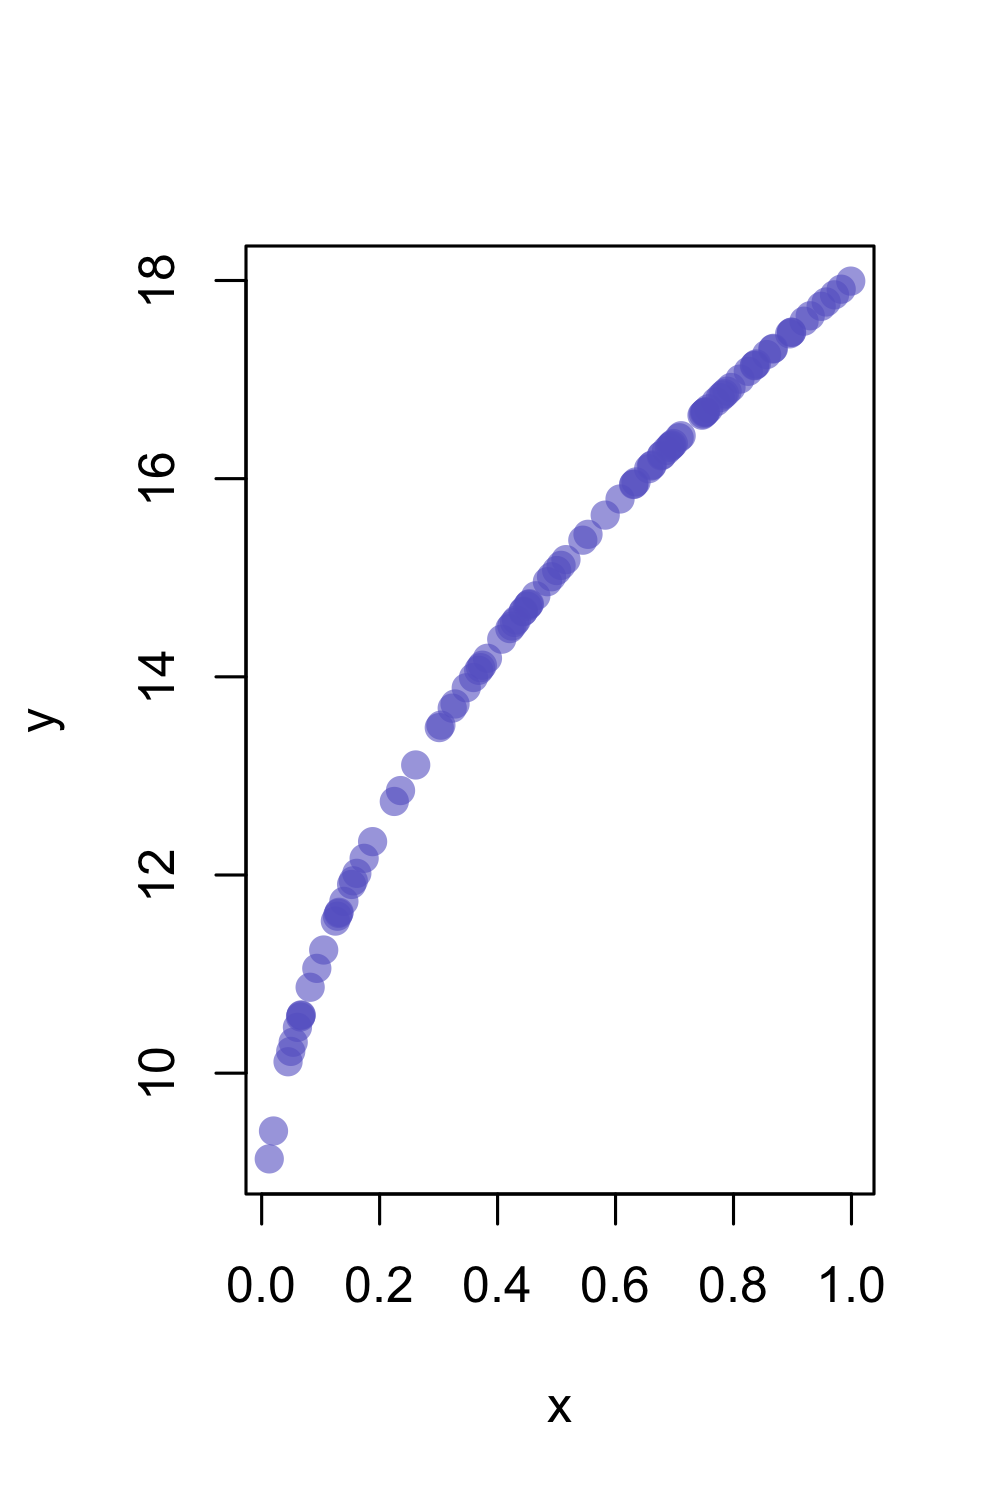
\includegraphics[width=.9\linewidth]{Ej7_poli.png}  
  \caption{$y = a * sqrt(x) + b$ }
  \label{sb1-1}
\end{subfigure}
\begin{subfigure}{.3\textwidth}
  \centering
  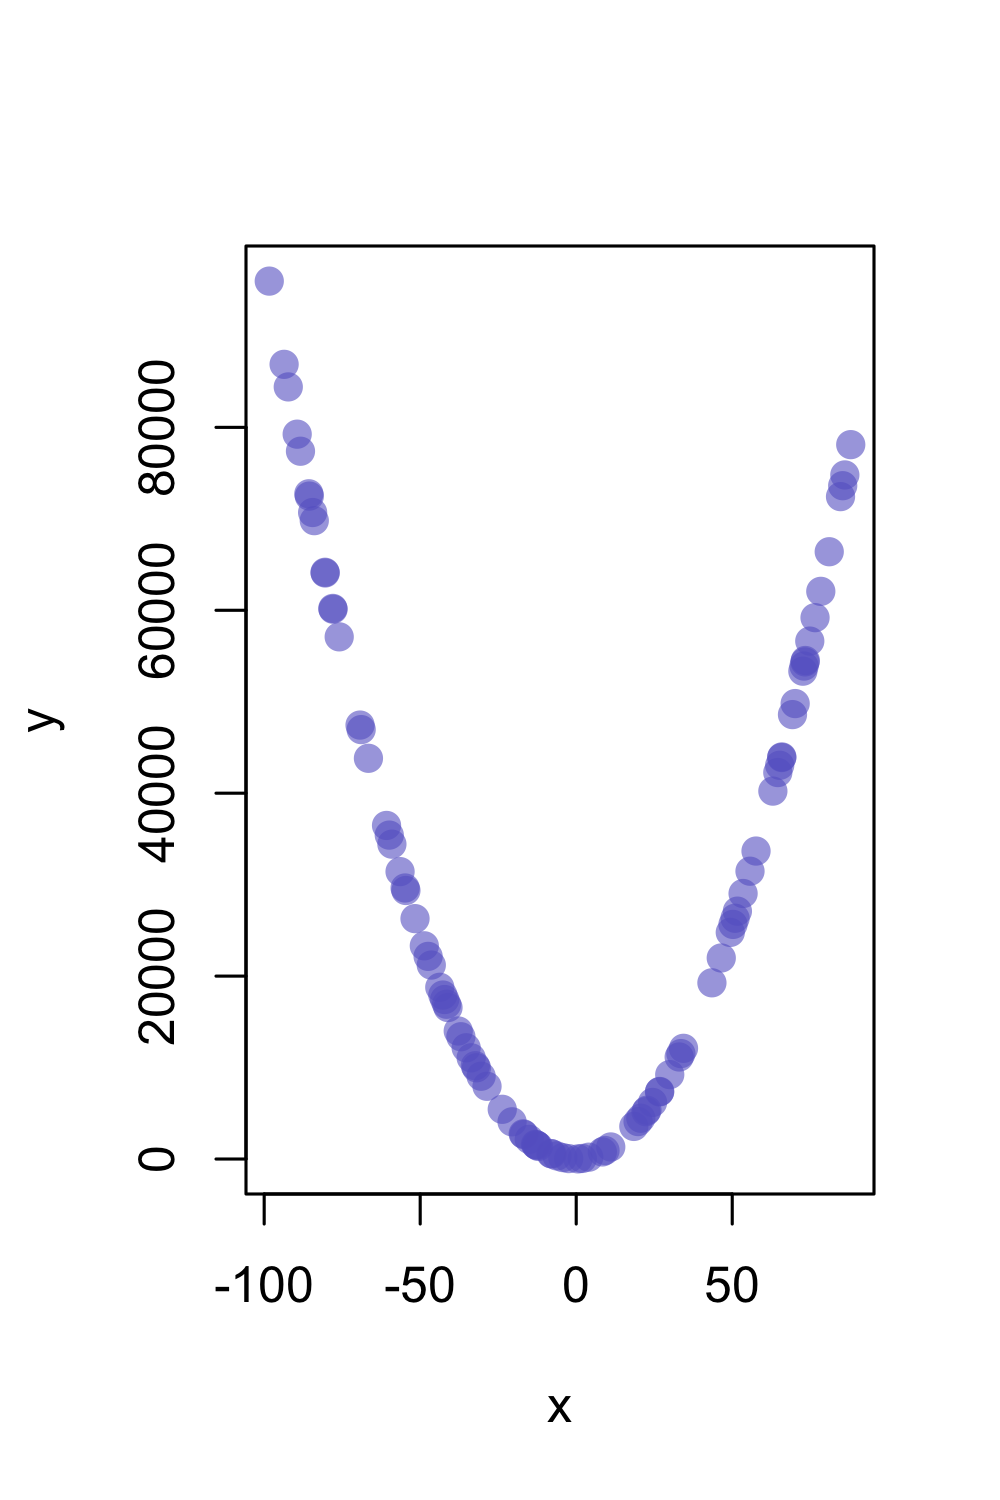
\includegraphics[width=.9\linewidth]{Ej7_cua.png}  
  \caption{$y = a*x^2 + b*x + c$}
  \label{sb1-2}
\end{subfigure}
\begin{subfigure}{.3\textwidth}
  \centering
  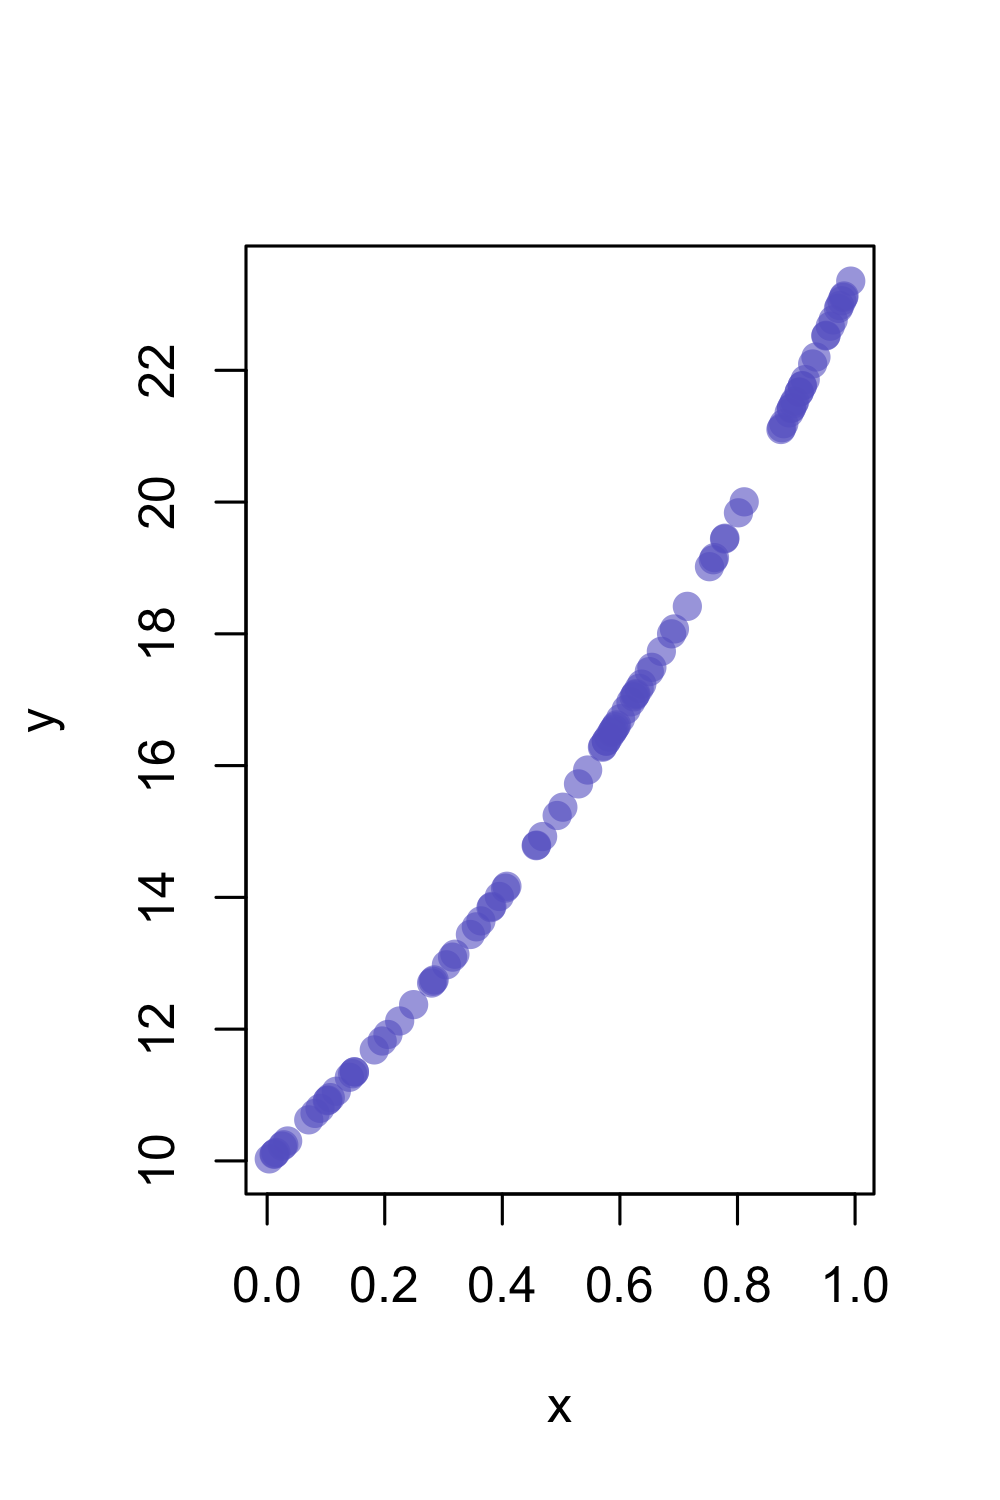
\includegraphics[width=.9\linewidth]{Ej7_exp.png}  
  \caption{$y = a * (exp(p * x))  $}
  \label{sb1-3}
\end{subfigure}
\newline
\begin{subfigure}{.5\textwidth}
  \centering
  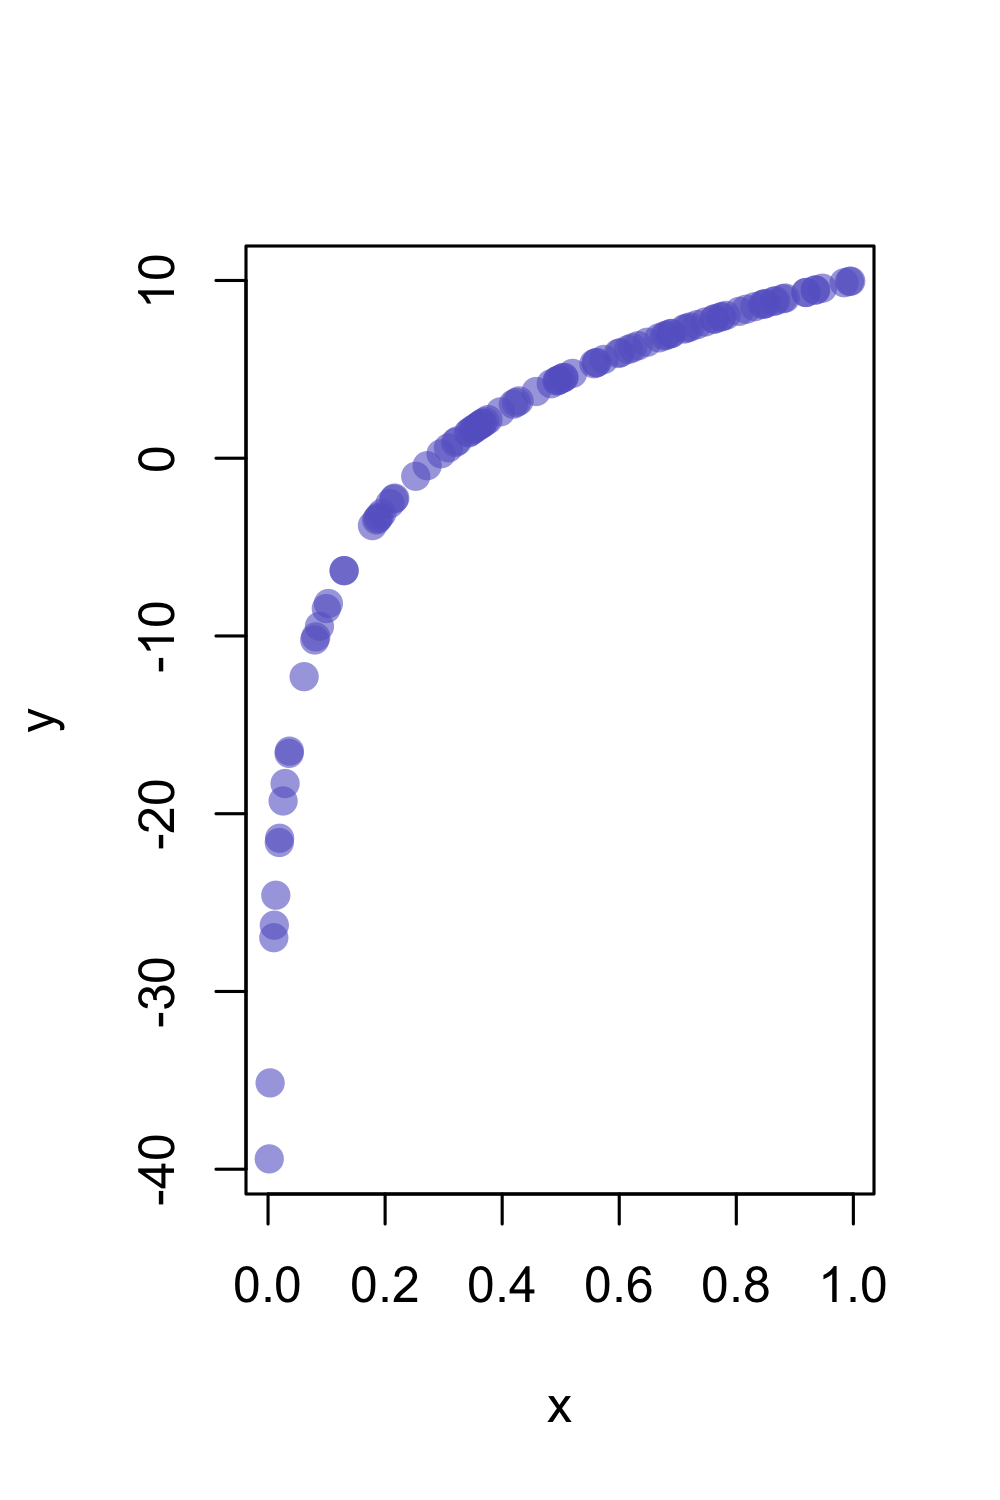
\includegraphics[width=.6\linewidth]{Ej7_log.png}  
  \caption{$y = a + b * log(x) $}
  \label{sb1-4}
\end{subfigure}
\begin{subfigure}{.5\textwidth}
  \centering
  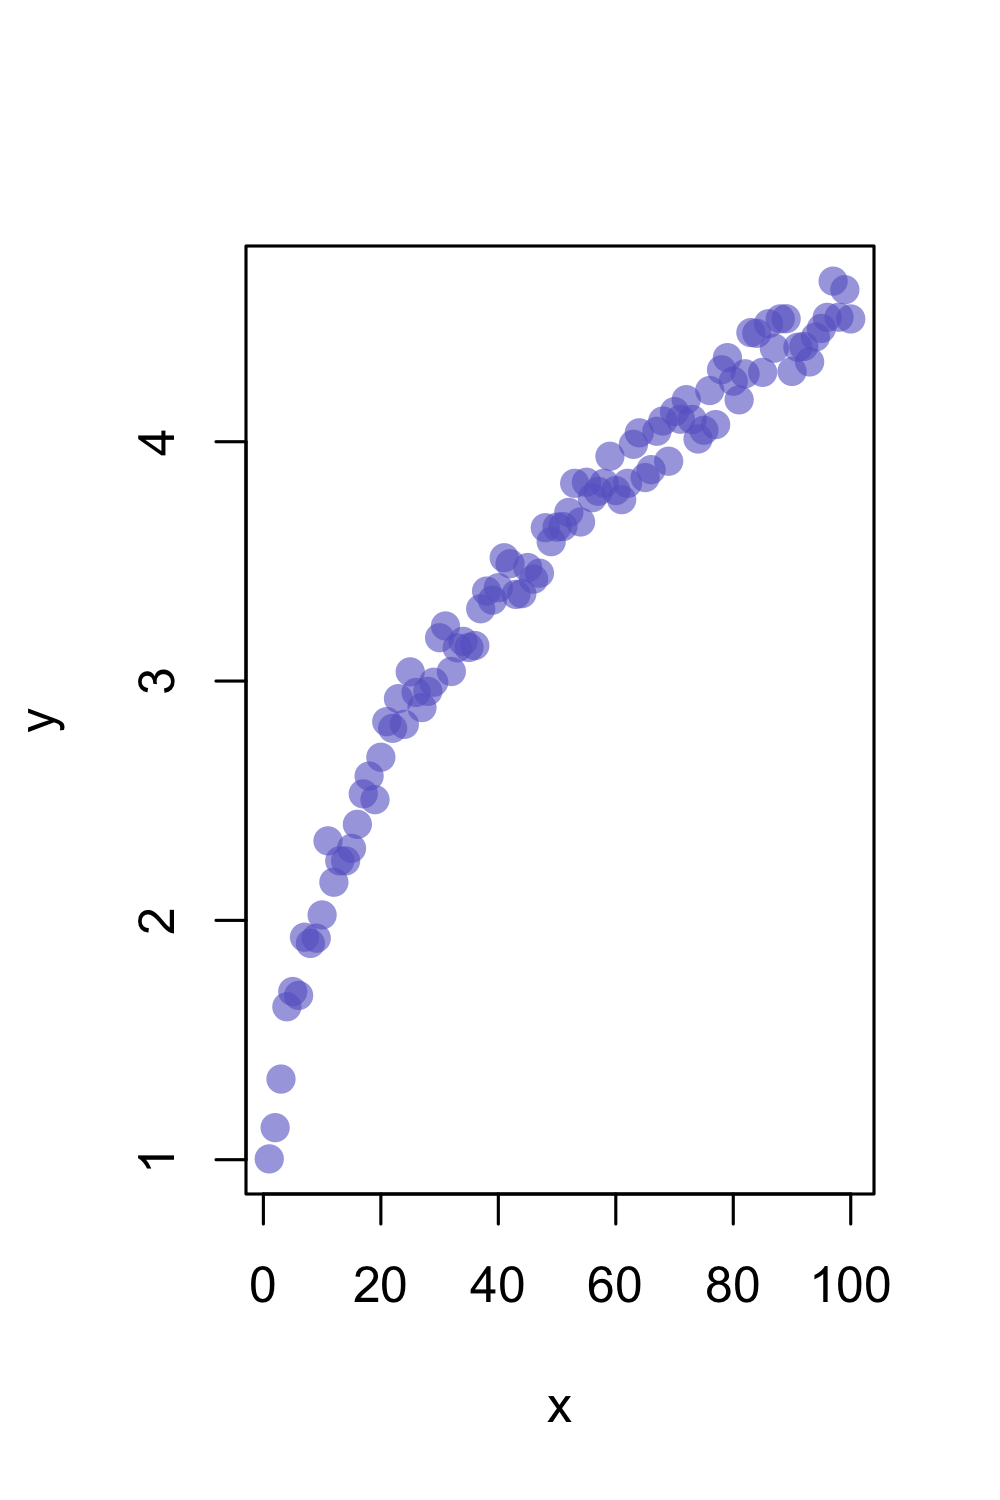
\includegraphics[width=.6\linewidth]{Ej7_jitter.png}  
  \caption{y = jitter$(x^p, factor = length(x)/2)$}
  \label{sb1-5}
\end{subfigure}
\caption{Scatter plots of each equation.}
\label{fig1}
\end{figure}

Visualization is a great tool to understand how some transformations work, so we use the \texttt{mosaic} and \texttt{manipulate} libraries in R to plot the behavior in each equation of the Tukey ladder of powers. \\

\clearpage

\subsection{Polynomial}\label{poly}

Polynomial equations are the most flexible tool to describe linear parameters, and can also be fitted with linear regression. The equation used in this part is Equation \ref{eq1}, 

\begin{equation} \label{eq1}
y =  a * sqrt(x) + b
\end{equation}
where:
\begin{description}
\item \texttt{a} and \texttt{b} are fixed variables,
\item \texttt{x} random uniform variable.
\end{description}

In Figure \ref{fig2} we can see the scatter plot of the equation \ref{sb2-1}, the residuals versus fitted values \ref{sb2-2}, and the normal Q-Q plot \ref{sb2-3}. We used both values of \texttt{x, y} to build a data frame. Then, we pretend that we do not now the fixed variables we put in the equation. With the plots in \ref{fig2} we can asees if the fit for a linear model is appropriate or not.\\

\begin{figure}[]
\begin{subfigure}{.3\textwidth}
  \centering
  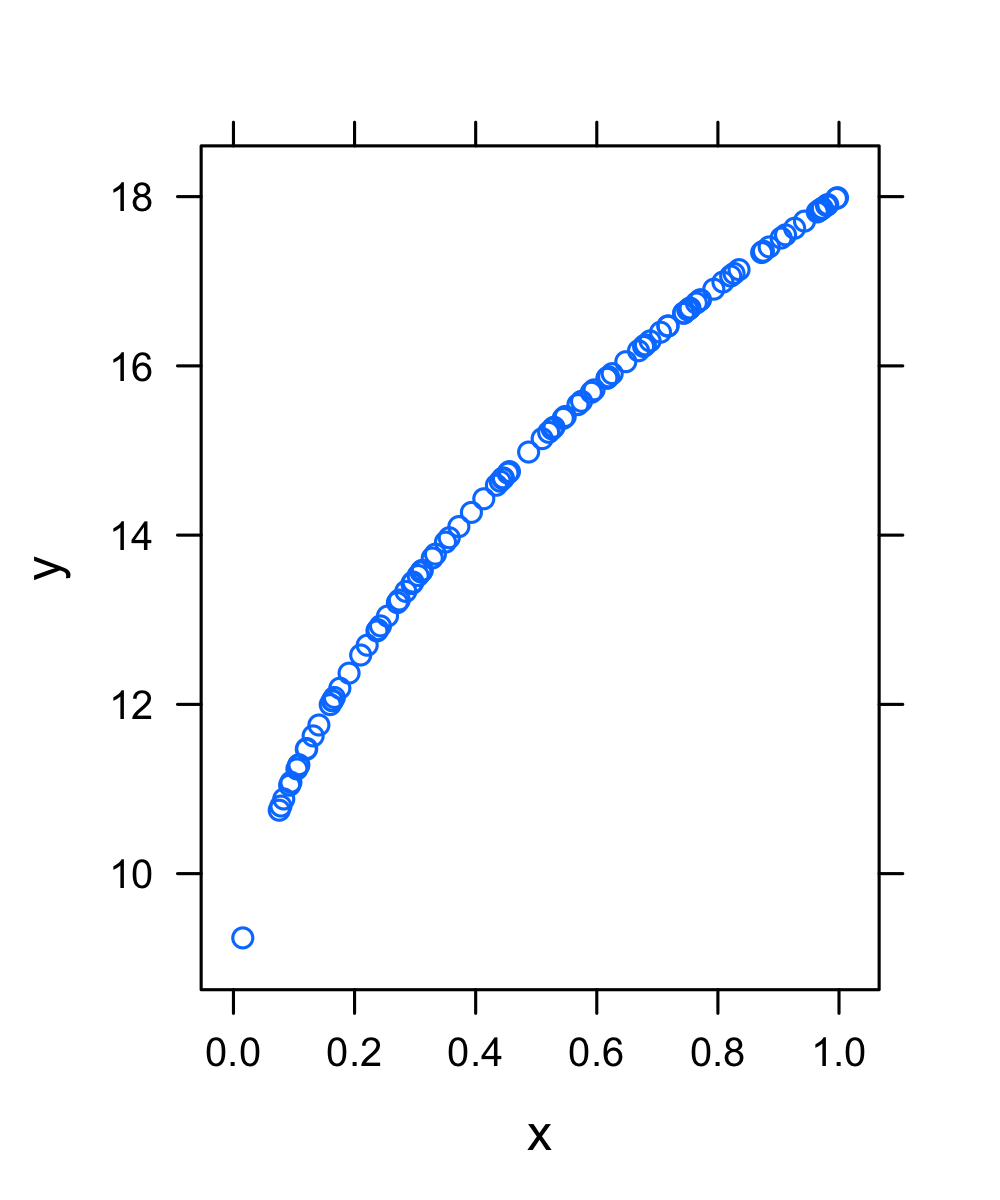
\includegraphics[width=.9\linewidth]{Ej7_p1-1.png}  
  \caption{ }
  \label{sb2-1}
\end{subfigure}
\begin{subfigure}{.3\textwidth}
  \centering
  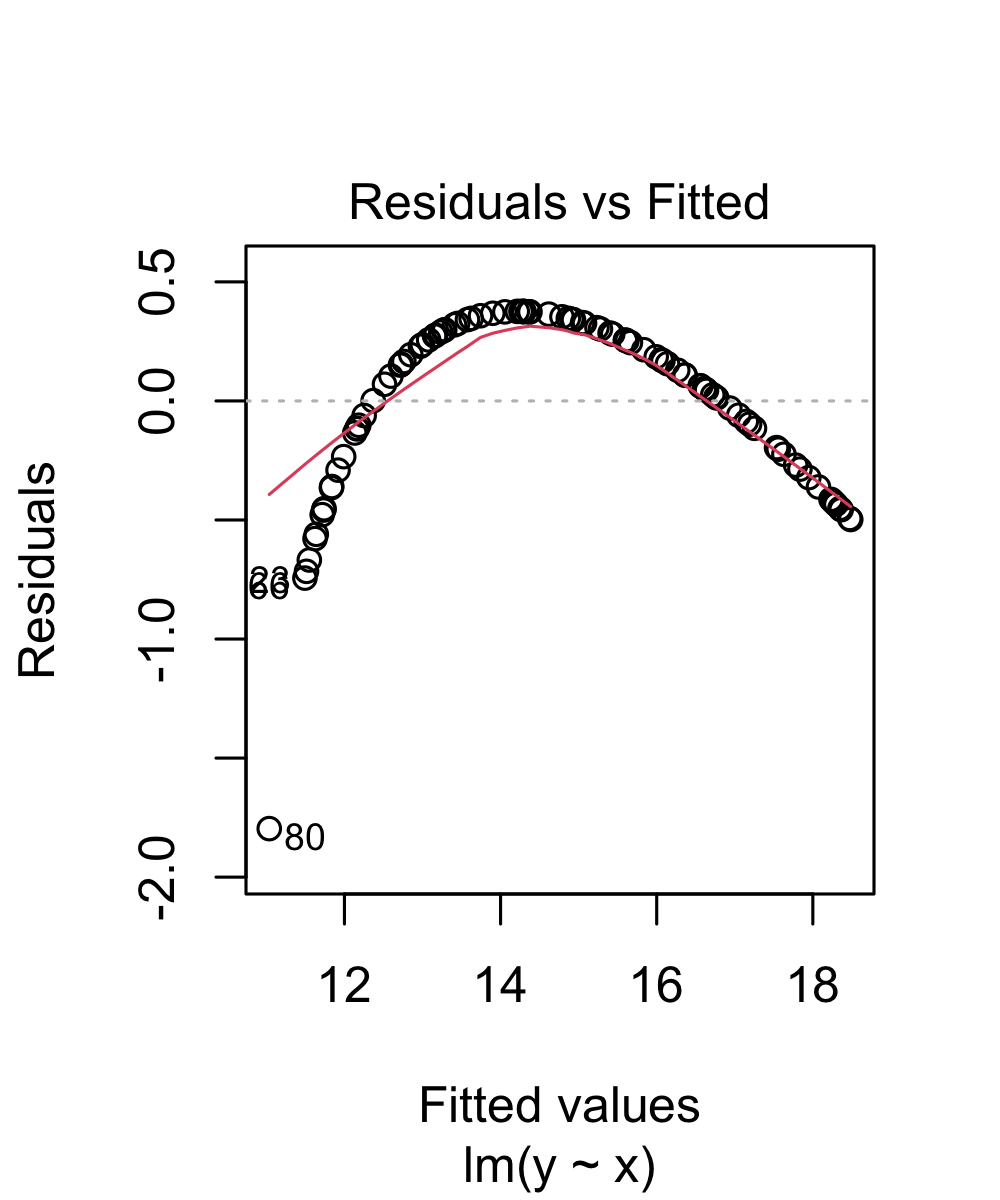
\includegraphics[width=.9\linewidth]{Ej7_p1-2.png}  
  \caption{ }
  \label{sb2-2}
\end{subfigure}
\begin{subfigure}{.3\textwidth}
  \centering
  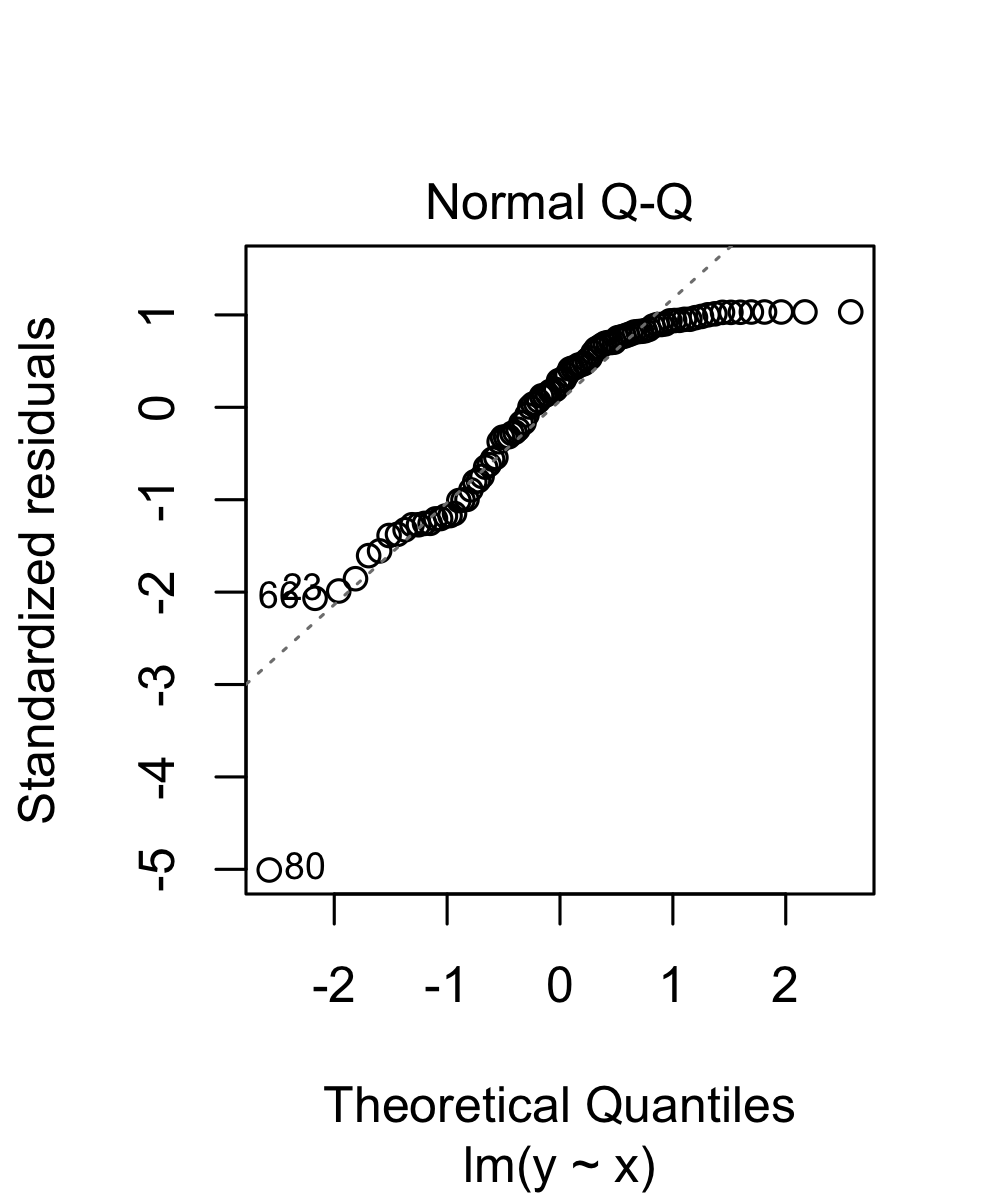
\includegraphics[width=.9\linewidth]{Ej7_p1-3.png}  
  \caption{ }
  \label{sb2-3}
\end{subfigure}
\caption{Scatter plot of equation (a), Residuals vs. Fitted plot (b), and Normal Q-Q plot (c) of polynomial equation.}
\label{fig2}
\end{figure}

As stated before, we are using the Tukey ladder of powers to determine an approximate transformation of the \texttt{y} variable. With the \texttt{manipulate} library in R we automate the process of searching for an appropriate value for lambda. Figure \ref{fig3} shows 13 iterations.\\

\begin{figure}[]
\begin{subfigure}{.23\textwidth}
  \centering
  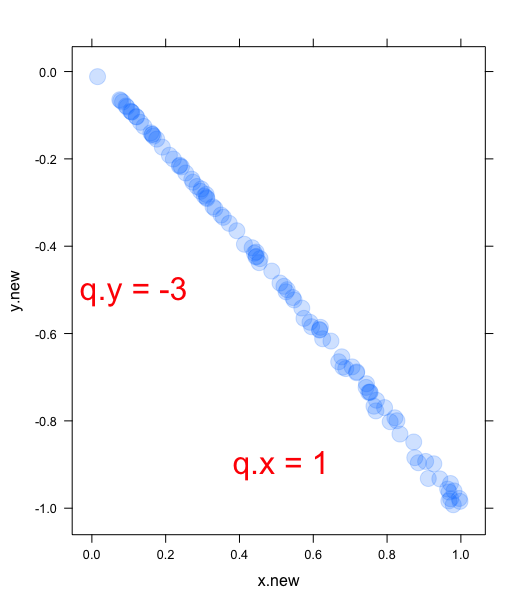
\includegraphics[width=.9\linewidth]{Ej7_1-1.png}  
  \caption{ }
  \label{sb3-1}
\end{subfigure}
\begin{subfigure}{.23\textwidth}
  \centering
  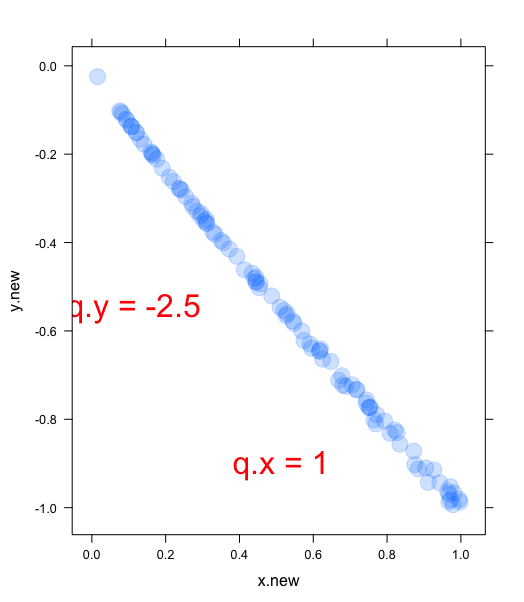
\includegraphics[width=.9\linewidth]{Ej7_1-2.png}  
  \caption{ }
  \label{sb3-2}
\end{subfigure}
\begin{subfigure}{.23\textwidth}
  \centering
  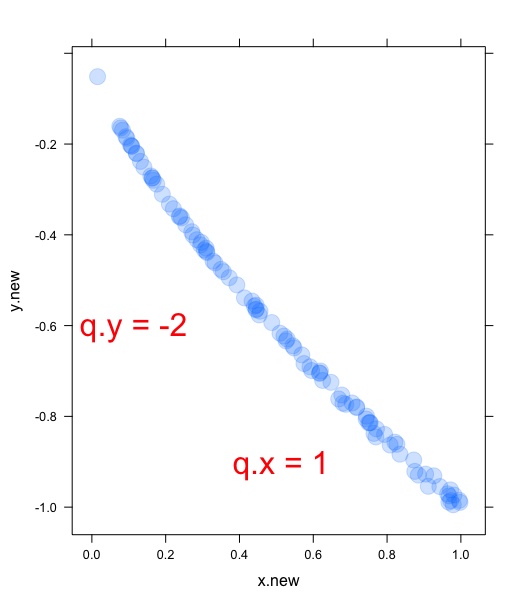
\includegraphics[width=.9\linewidth]{Ej7_1-3.png}  
  \caption{ }
  \label{sb3-3}
\end{subfigure}
\begin{subfigure}{.23\textwidth}
  \centering
  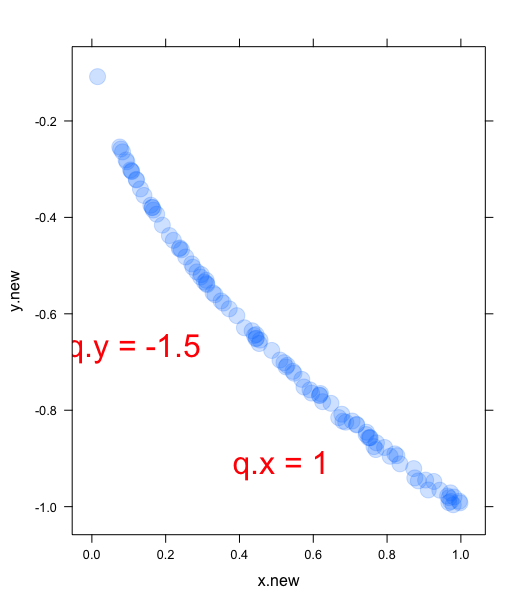
\includegraphics[width=.9\linewidth]{Ej7_1-4.png}  
  \caption{ }
  \label{sb3-4}
\end{subfigure}
\newline
\begin{subfigure}{.23\textwidth}
  \centering
  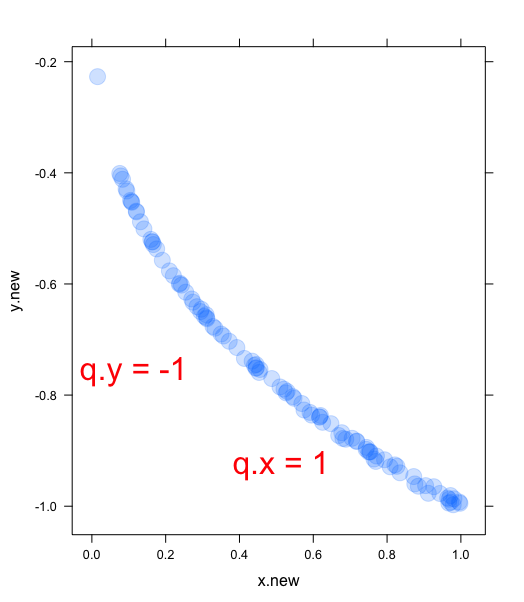
\includegraphics[width=.9\linewidth]{Ej7_1-5.png}  
  \caption{ }
  \label{sb3-5}
\end{subfigure}
\begin{subfigure}{.23\textwidth}
  \centering
  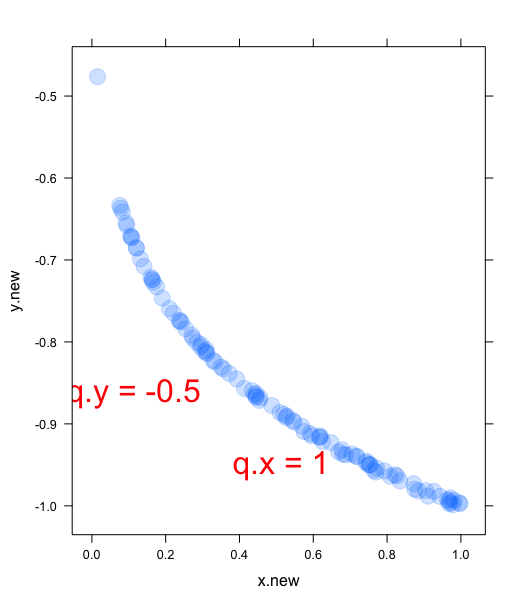
\includegraphics[width=.9\linewidth]{Ej7_1-6.png}  
  \caption{ }
  \label{sb3-6}
\end{subfigure}
\begin{subfigure}{.23\textwidth}
  \centering
  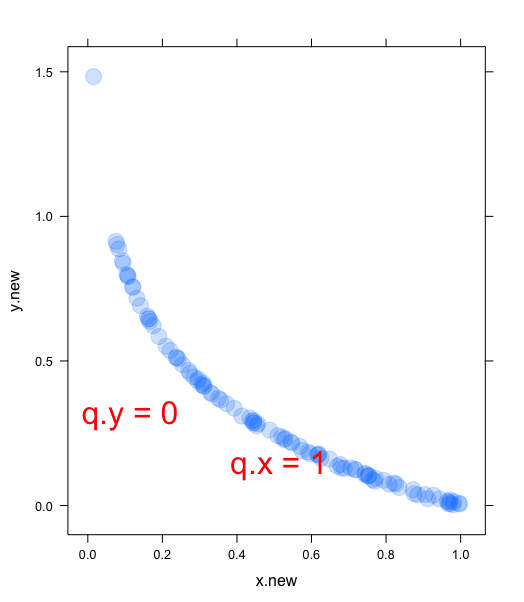
\includegraphics[width=.9\linewidth]{Ej7_1-7.png}  
  \caption{ }
  \label{sb3-7}
\end{subfigure}
\begin{subfigure}{.23\textwidth}
  \centering
  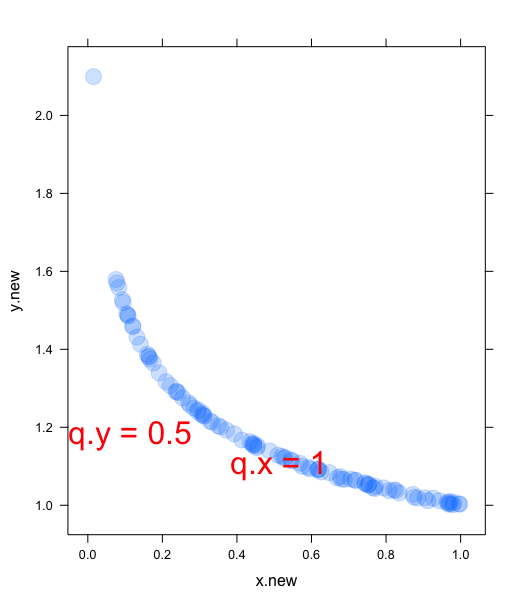
\includegraphics[width=.9\linewidth]{Ej7_1-8.png}  
  \caption{ }
  \label{sb3-8}
\end{subfigure}
\newline
\begin{subfigure}{.23\textwidth}
  \centering
  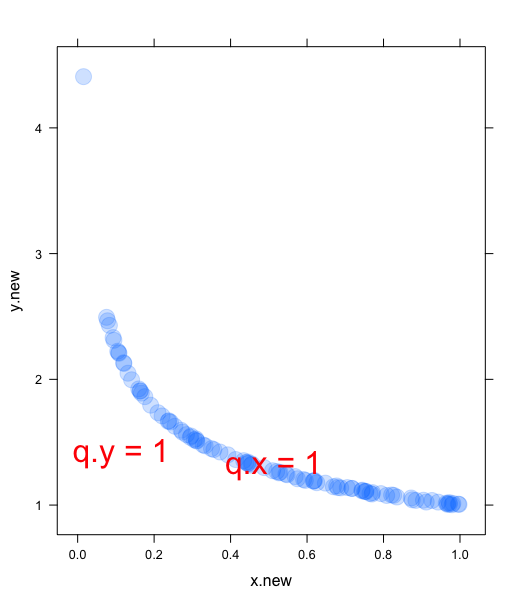
\includegraphics[width=.9\linewidth]{Ej7_1-9.png}  
  \caption{ }
  \label{sb3-9}
\end{subfigure}
\begin{subfigure}{.23\textwidth}
  \centering
  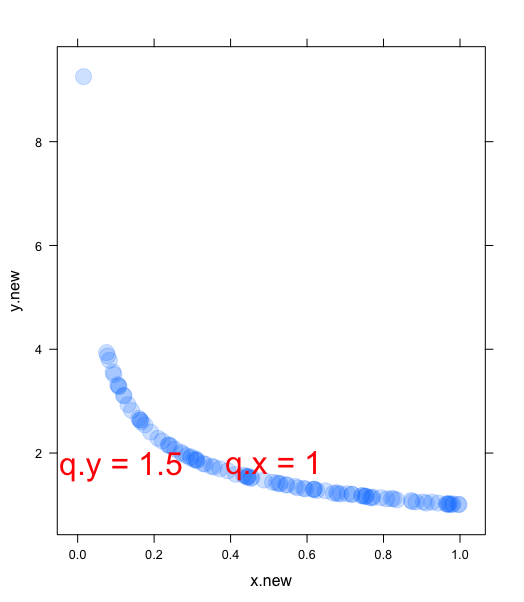
\includegraphics[width=.9\linewidth]{Ej7_1-10.png}  
  \caption{ }
  \label{sb3-10}
\end{subfigure}
\begin{subfigure}{.23\textwidth}
  \centering
  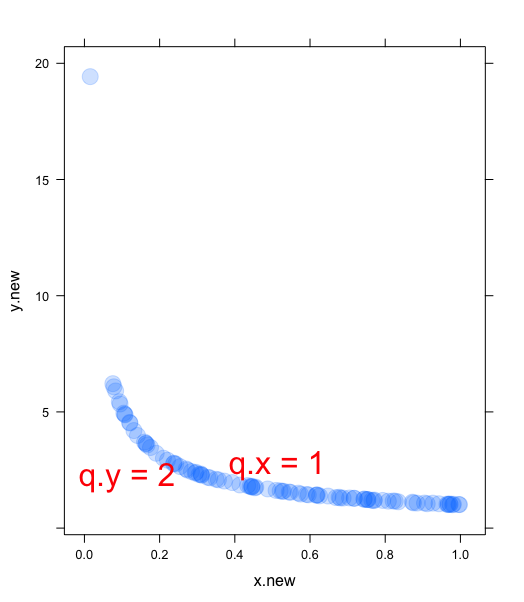
\includegraphics[width=.9\linewidth]{Ej7_1-11.png}  
  \caption{ }
  \label{sb3-11}
\end{subfigure}
\begin{subfigure}{.23\textwidth}
  \centering
  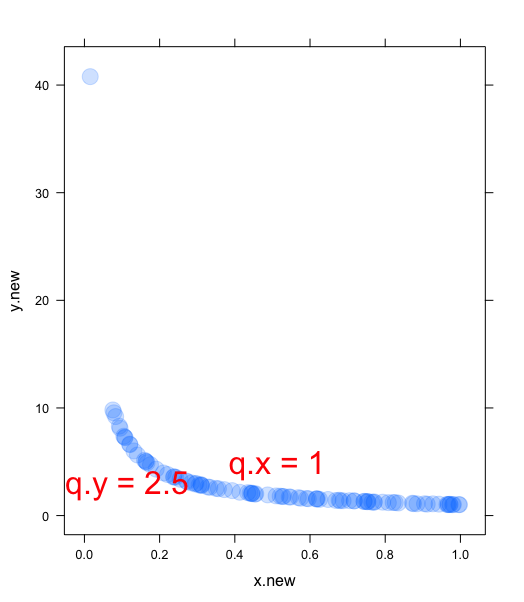
\includegraphics[width=.9\linewidth]{Ej7_1-12.png}  
  \caption{ }
  \label{sb3-12}
\end{subfigure}
\newline
\begin{subfigure}{1\textwidth}
  \centering
  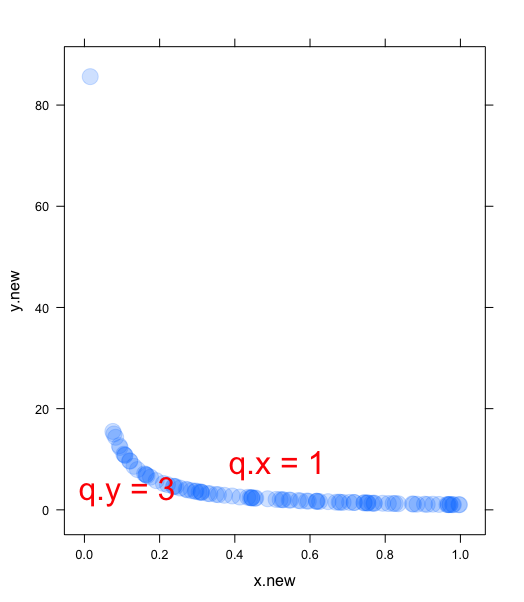
\includegraphics[width=.22\linewidth]{Ej7_1-13.png}  
  \caption{ }
  \label{sb3-13}
\end{subfigure}
\caption{Iterations of the different values of lambda for the Tukey ladder of powers for the polynomial equation.}
\label{fig3}
\end{figure}

The best fit for a linear model is Figure \ref{sb3-1} with $\lambda$= -3.\\

\clearpage


\subsection{Quadratic}

The equation used for this is Equation \ref{eq2}, 

\begin{equation} \label{eq2}
y =  a*x^2 + b*x + c 
\end{equation}

where all the fixed values are the same as the one used in Section \ref{poly}.\\

\begin{figure}[]
\begin{subfigure}{.3\textwidth}
  \centering
  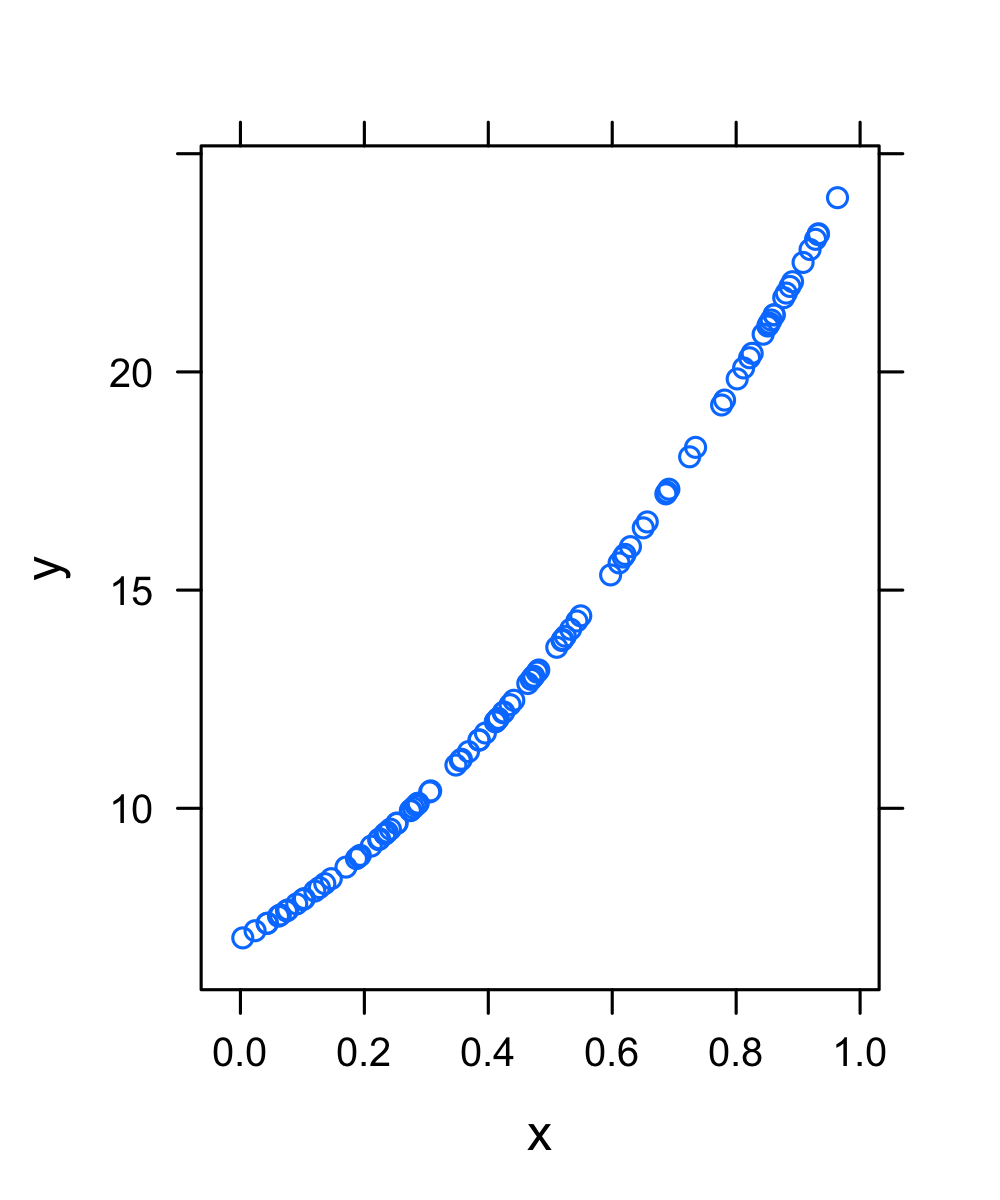
\includegraphics[width=.9\linewidth]{Ej7_p2-1.png}  
  \caption{ }
  \label{sb4-1}
\end{subfigure}
\begin{subfigure}{.3\textwidth}
  \centering
  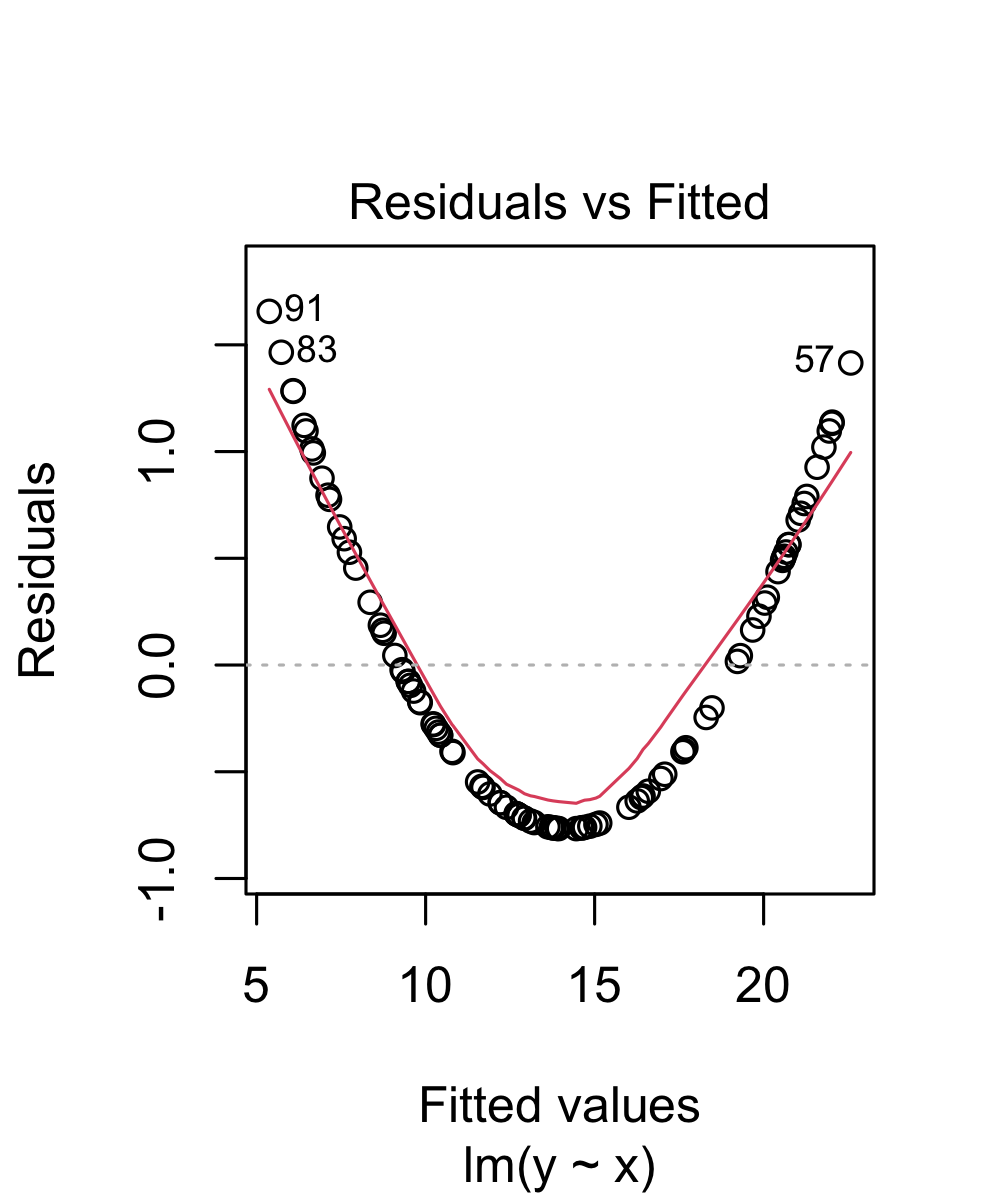
\includegraphics[width=.9\linewidth]{Ej7_p2-2.png}  
  \caption{ }
  \label{sb4-2}
\end{subfigure}
\begin{subfigure}{.3\textwidth}
  \centering
  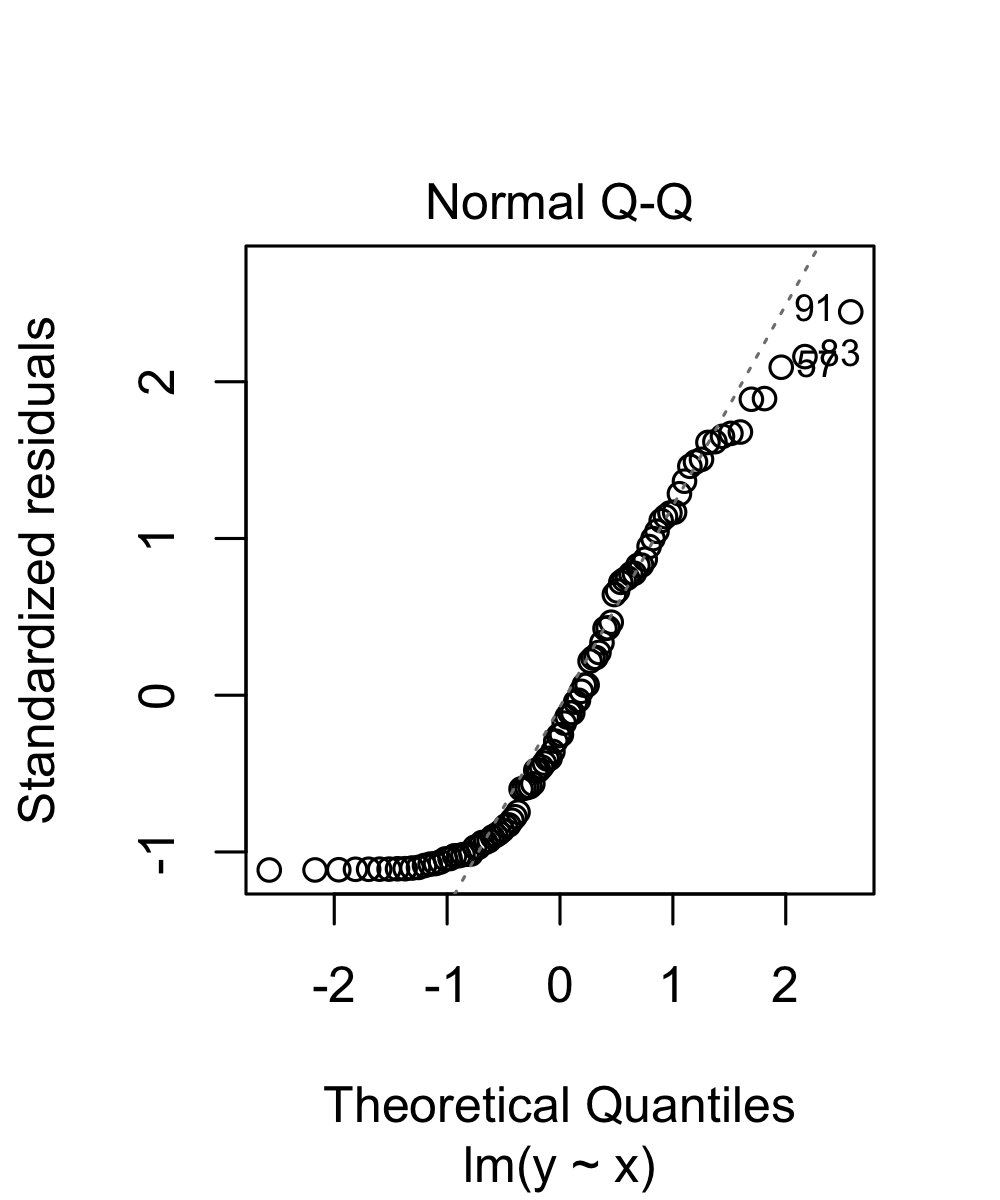
\includegraphics[width=.9\linewidth]{Ej7_p2-3.png}  
  \caption{ }
  \label{sb4-3}
\end{subfigure}
\caption{Scatter plot of equation (a), Residuals vs. Fitted plot (b), and Normal Q-Q plot (c) of quadratic equation.}
\label{fig4}
\end{figure}

In Figure \ref{fig5} we have the iterations of the Tukey ladder. Examining this plot, Figure \ref{sb5-9} is the one that shows a linear behaviour. In this case, $\lambda$ = 1.\\

\begin{figure}[]
\begin{subfigure}{.23\textwidth}
  \centering
  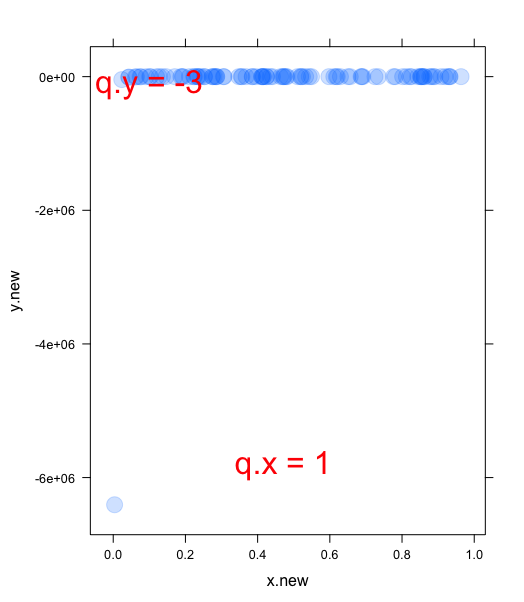
\includegraphics[width=.9\linewidth]{Ej7_2-1.png}  
  \caption{ }
  \label{sb5-1}
\end{subfigure}
\begin{subfigure}{.23\textwidth}
  \centering
  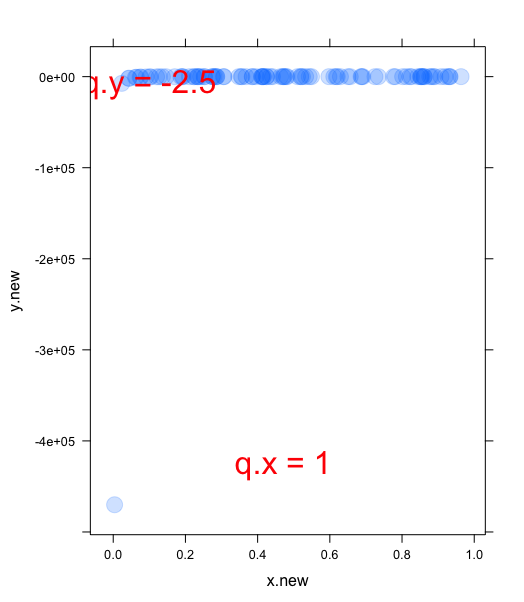
\includegraphics[width=.9\linewidth]{Ej7_2-2.png}  
  \caption{ }
  \label{sb5-2}
\end{subfigure}
\begin{subfigure}{.23\textwidth}
  \centering
  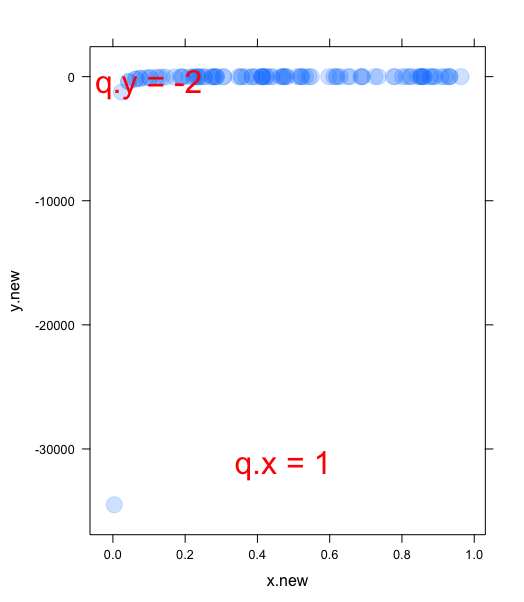
\includegraphics[width=.9\linewidth]{Ej7_2-3.png}  
  \caption{ }
  \label{sb5-3}
\end{subfigure}
\begin{subfigure}{.23\textwidth}
  \centering
  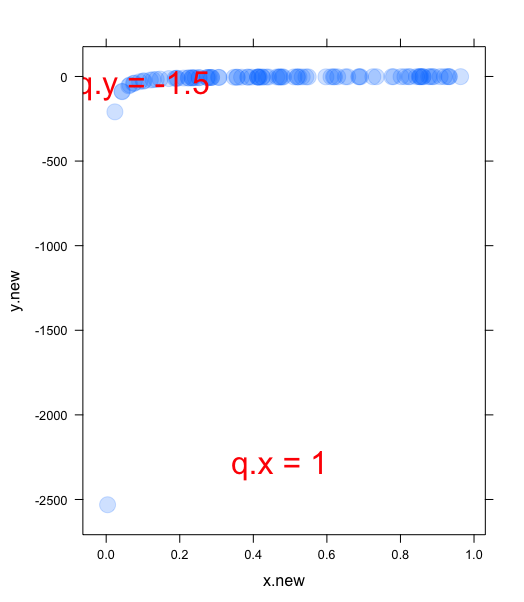
\includegraphics[width=.9\linewidth]{Ej7_2-4.png}  
  \caption{ }
  \label{sb5-4}
\end{subfigure}
\newline
\begin{subfigure}{.23\textwidth}
  \centering
  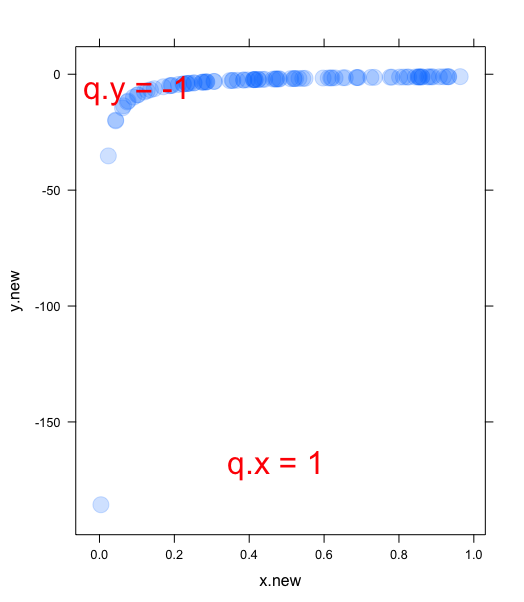
\includegraphics[width=.9\linewidth]{Ej7_2-5.png}  
  \caption{ }
  \label{sb5-5}
\end{subfigure}
\begin{subfigure}{.23\textwidth}
  \centering
  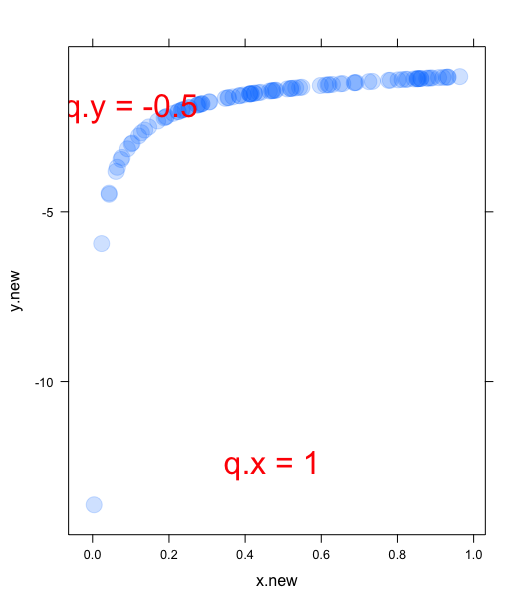
\includegraphics[width=.9\linewidth]{Ej7_2-6.png}  
  \caption{ }
  \label{sb5-6}
\end{subfigure}
\begin{subfigure}{.23\textwidth}
  \centering
  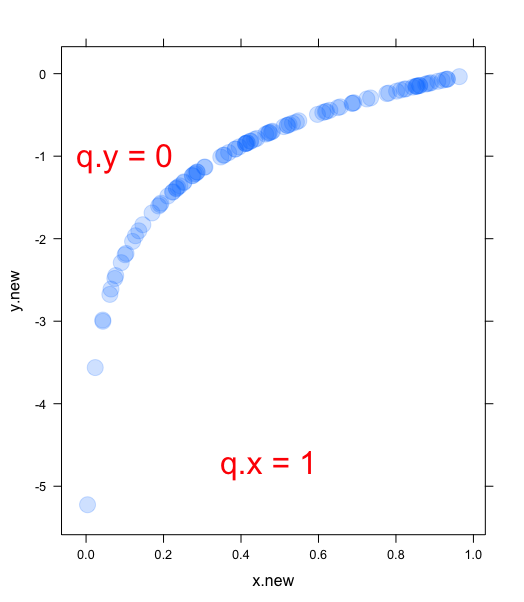
\includegraphics[width=.9\linewidth]{Ej7_2-7.png}  
  \caption{ }
  \label{sb5-7}
\end{subfigure}
\begin{subfigure}{.23\textwidth}
  \centering
  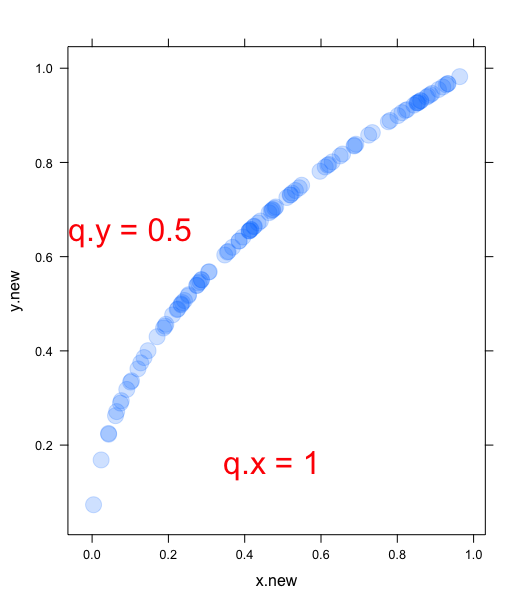
\includegraphics[width=.9\linewidth]{Ej7_2-8.png}  
  \caption{ }
  \label{sb5-8}
\end{subfigure}
\newline
\begin{subfigure}{.23\textwidth}
  \centering
  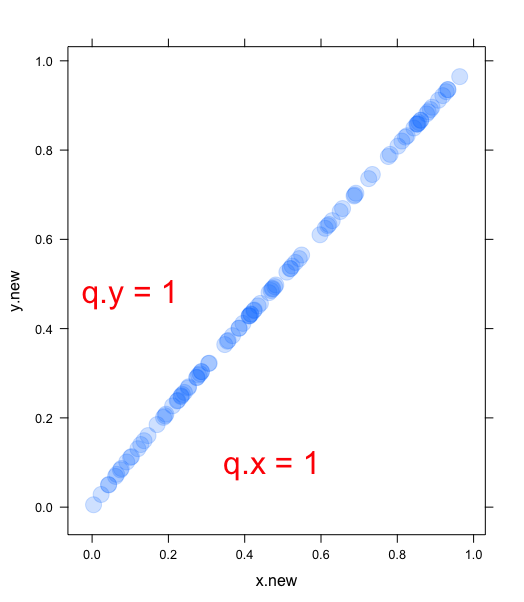
\includegraphics[width=.9\linewidth]{Ej7_2-9.png}  
  \caption{ }
  \label{sb5-9}
\end{subfigure}
\begin{subfigure}{.23\textwidth}
  \centering
  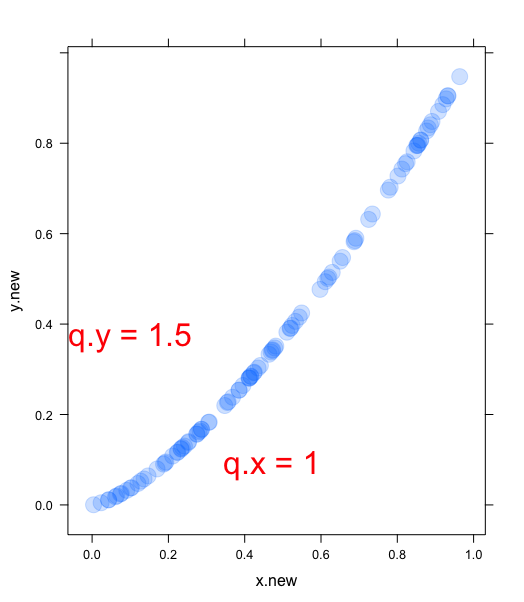
\includegraphics[width=.9\linewidth]{Ej7_2-10.png}  
  \caption{ }
  \label{sb5-10}
\end{subfigure}
\begin{subfigure}{.23\textwidth}
  \centering
  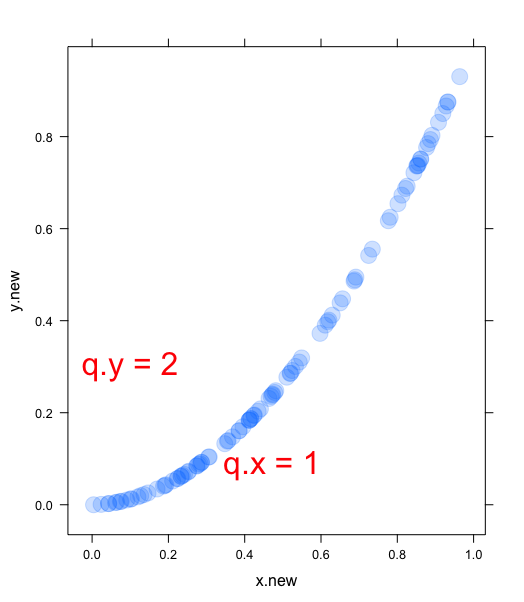
\includegraphics[width=.9\linewidth]{Ej7_2-11.png}  
  \caption{ }
  \label{sb5-11}
\end{subfigure}
\begin{subfigure}{.23\textwidth}
  \centering
  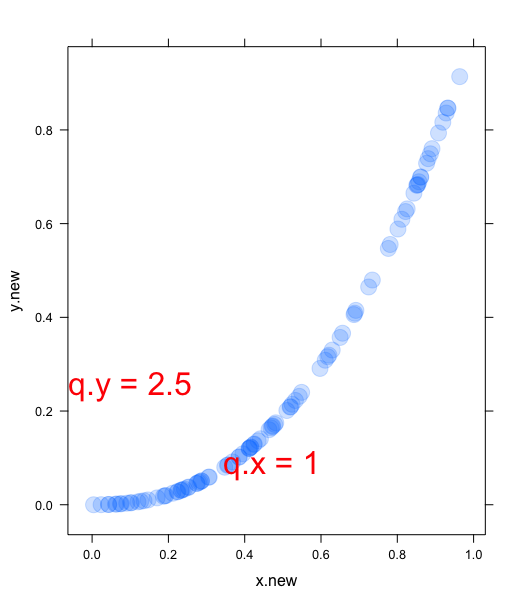
\includegraphics[width=.9\linewidth]{Ej7_2-12.png}  
  \caption{ }
  \label{sb5-12}
\end{subfigure}
\newline
\begin{subfigure}{1\textwidth}
  \centering
  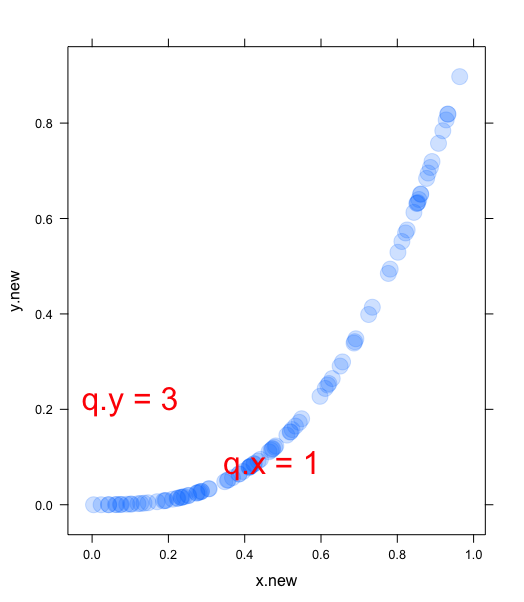
\includegraphics[width=.22\linewidth]{Ej7_2-13.png}  
  \caption{ }
  \label{sb5-13}
\end{subfigure}
\caption{Iterations of the different values of lambda for the Tukey ladder of powers for the quadratic equation.}
\label{fig5}
\end{figure}

\clearpage

\subsection{Exponential}

In the case of the exponential equation, it describes an increasing or decreasing trend, with a constant relative rate. Equation \ref{eq3} shows the parameters used, 

\begin{equation} \label{eq3}
y = a * (exp(p * x))
\end{equation}

where all the constant variables are the same used in the polinomial and quadratic equations. The value of \texttt{p} is a standard normal random variable.\\

\begin{figure}[]
\begin{subfigure}{.3\textwidth}
  \centering
  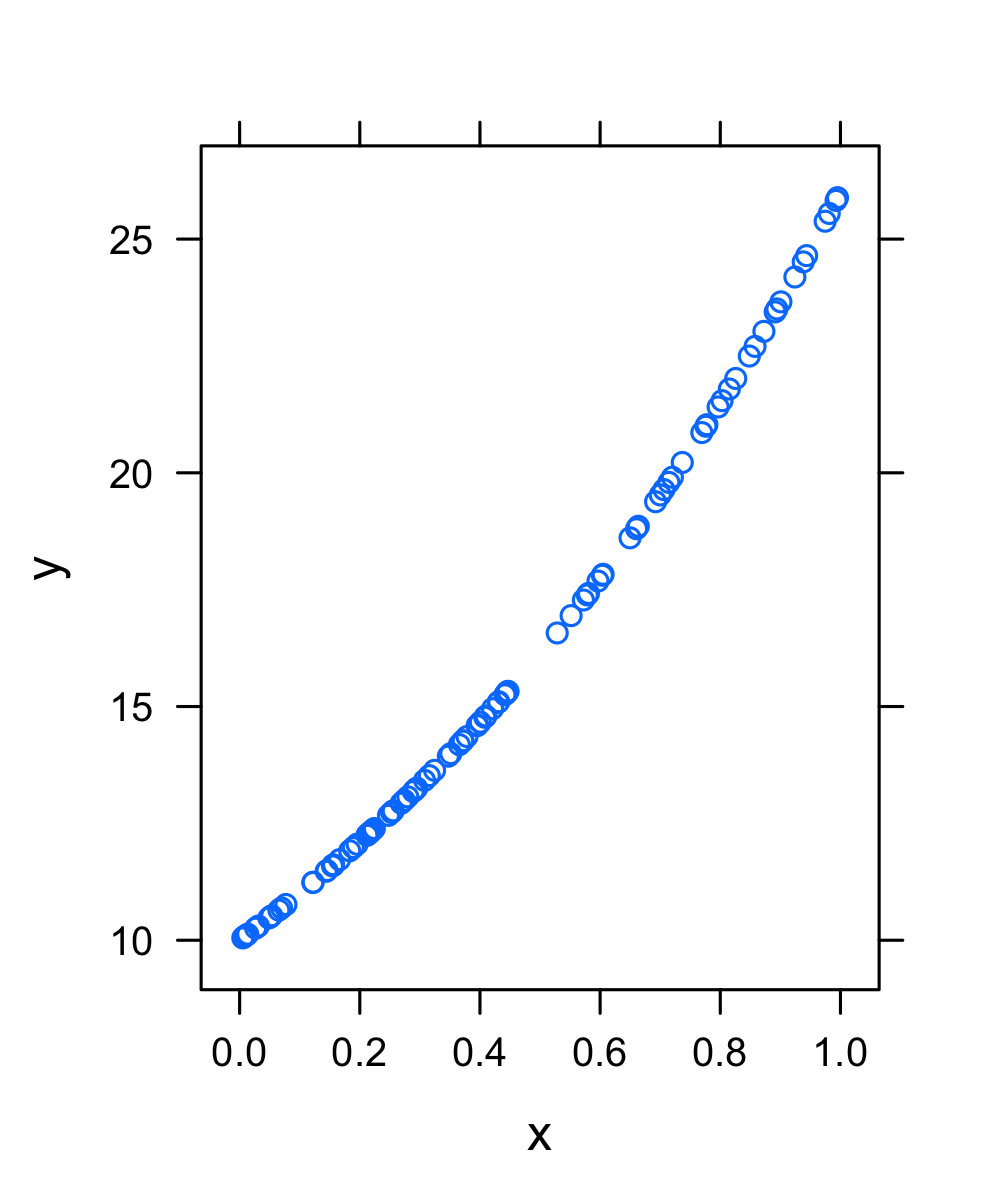
\includegraphics[width=.9\linewidth]{Ej7_p3-1.png}  
  \caption{$y = a * sqrt(x) + b$ }
  \label{sb6-1}
\end{subfigure}
\begin{subfigure}{.3\textwidth}
  \centering
  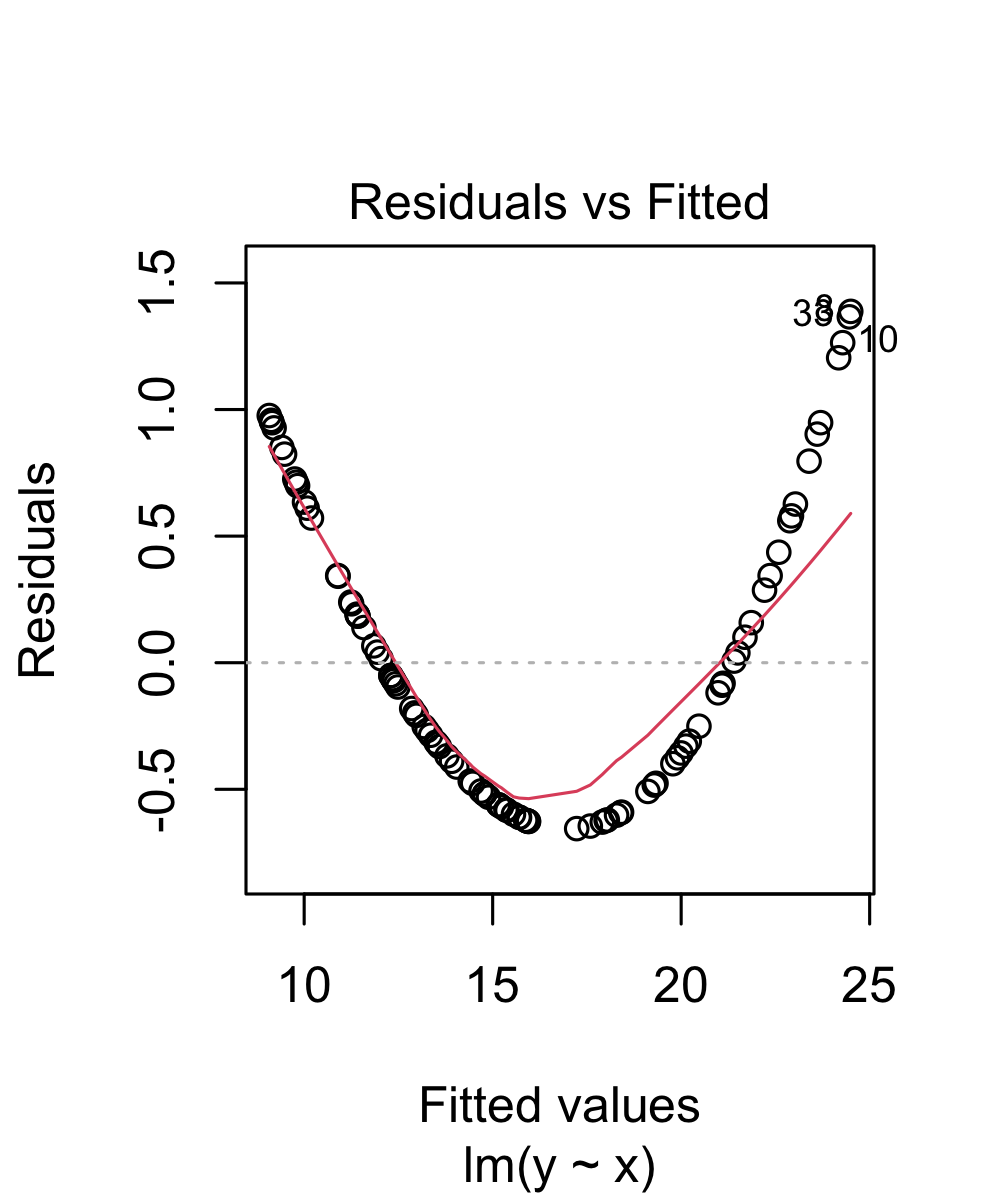
\includegraphics[width=.9\linewidth]{Ej7_p3-2.png}  
  \caption{$y = a*x^2 + b*x + c$}
  \label{sb6-2}
\end{subfigure}
\begin{subfigure}{.3\textwidth}
  \centering
  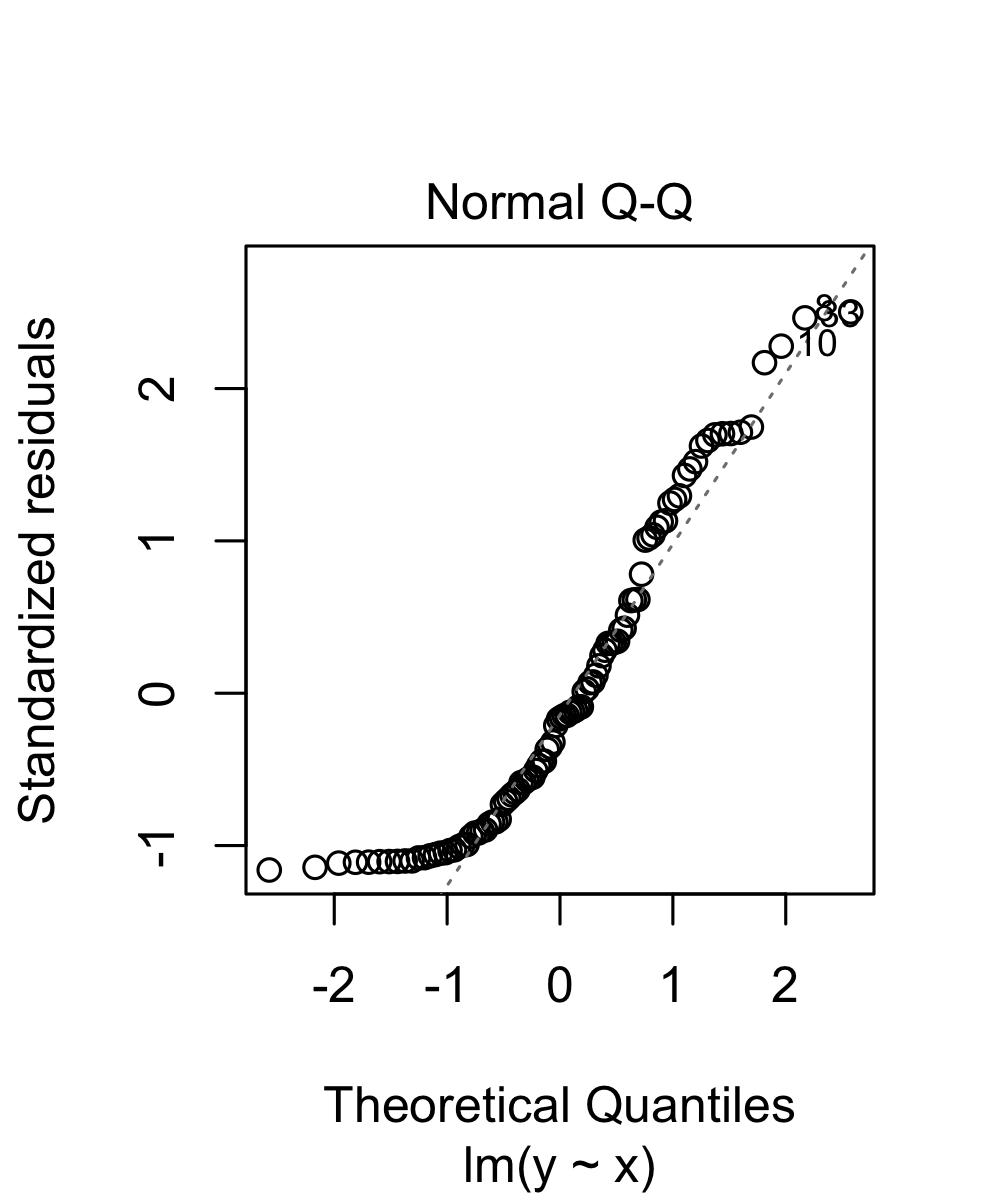
\includegraphics[width=.9\linewidth]{Ej7_p3-3.png}  
  \caption{$y = a * (exp(p * x))  $}
  \label{sb6-3}
\end{subfigure}
\caption{Scatter plot of equation (a), Residuals vs. Fitted plot (b), and Normal Q-Q plot (c) of exponential equation.}
\label{fig6}
\end{figure}

\begin{figure}[]
\begin{subfigure}{.23\textwidth}
  \centering
  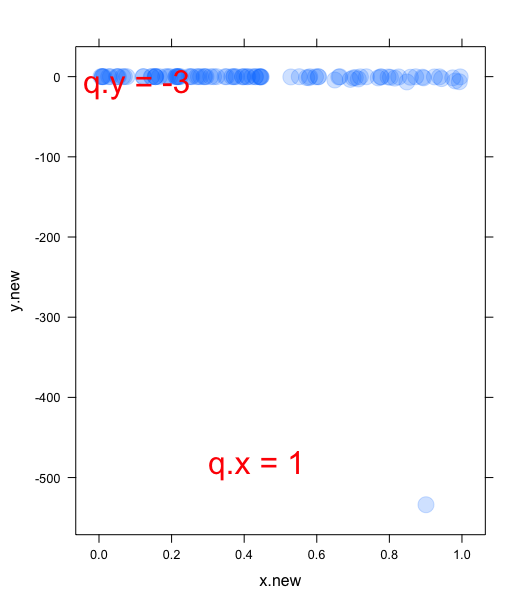
\includegraphics[width=.9\linewidth]{E7_3-1.png}  
  \caption{ }
  \label{sb7-1}
\end{subfigure}
\begin{subfigure}{.23\textwidth}
  \centering
  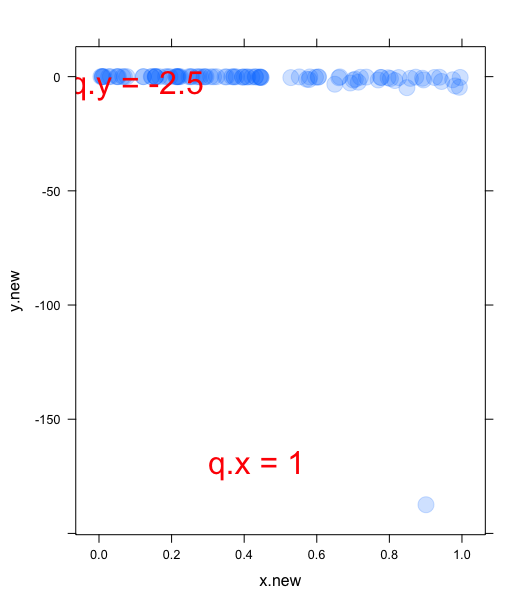
\includegraphics[width=.9\linewidth]{E7_3-2.png}  
  \caption{ }
  \label{sb7-2}
\end{subfigure}
\begin{subfigure}{.23\textwidth}
  \centering
  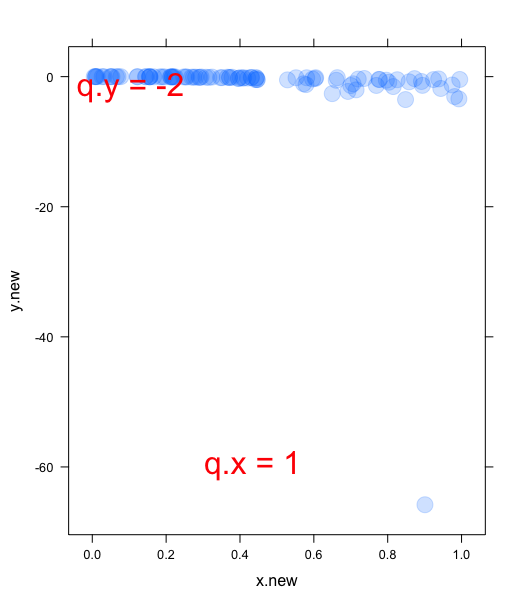
\includegraphics[width=.9\linewidth]{E7_3-3.png}  
  \caption{ }
  \label{sb7-3}
\end{subfigure}
\begin{subfigure}{.23\textwidth}
  \centering
  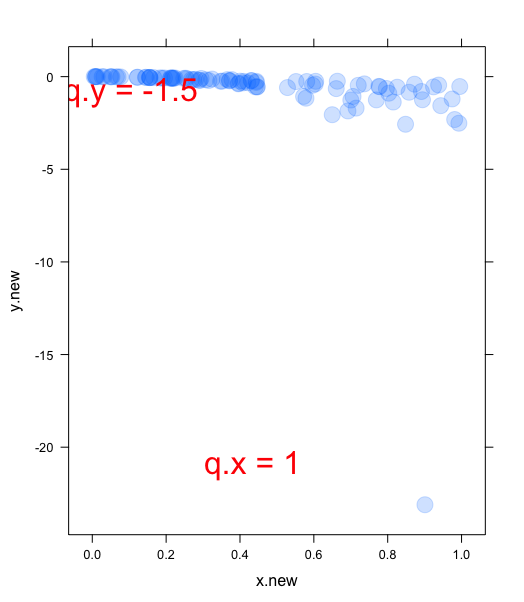
\includegraphics[width=.9\linewidth]{E7_3-4.png}  
  \caption{ }
  \label{sb7-4}
\end{subfigure}
\newline
\begin{subfigure}{.23\textwidth}
  \centering
  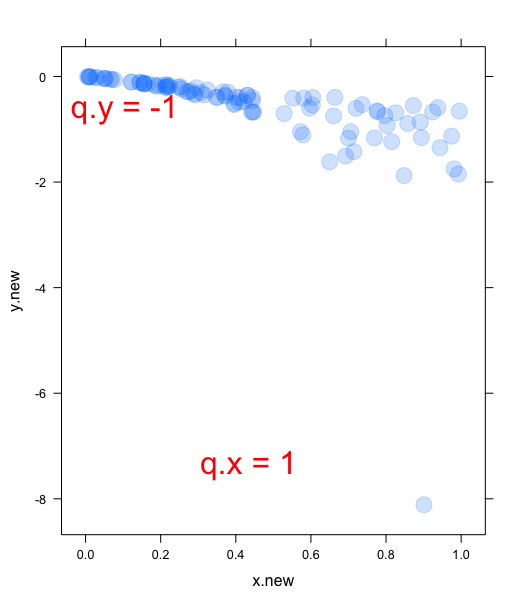
\includegraphics[width=.9\linewidth]{E7_3-5.png}  
  \caption{ }
  \label{sb7-5}
\end{subfigure}
\begin{subfigure}{.23\textwidth}
  \centering
  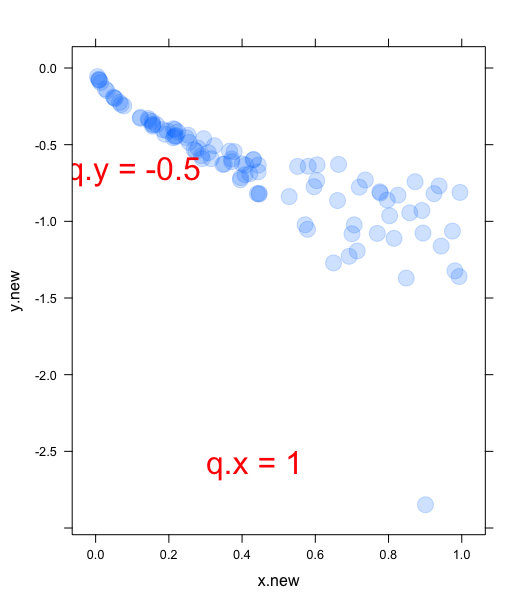
\includegraphics[width=.9\linewidth]{E7_3-6.png}  
  \caption{ }
  \label{sb7-6}
\end{subfigure}
\begin{subfigure}{.23\textwidth}
  \centering
  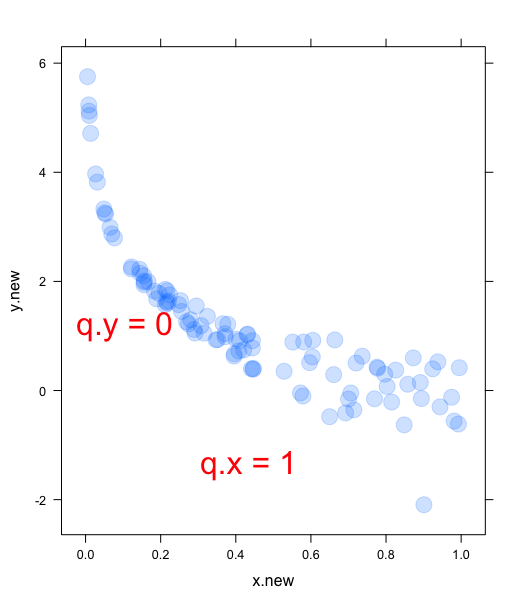
\includegraphics[width=.9\linewidth]{E7_3-7.png}  
  \caption{ }
  \label{sb7-7}
\end{subfigure}
\begin{subfigure}{.23\textwidth}
  \centering
  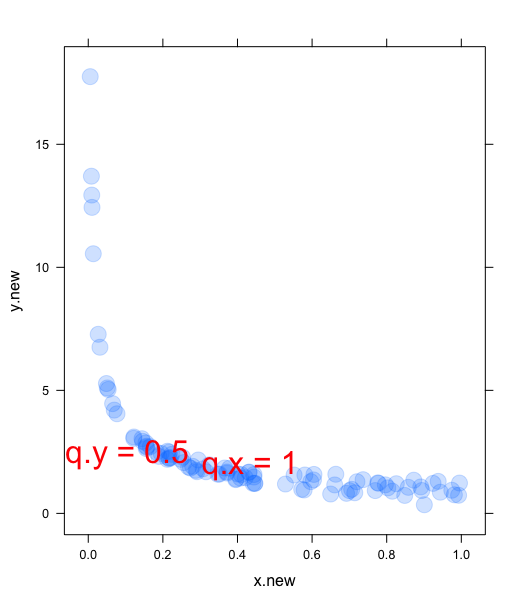
\includegraphics[width=.9\linewidth]{E7_3-8.png}  
  \caption{ }
  \label{sb7-8}
\end{subfigure}
\newline
\begin{subfigure}{.23\textwidth}
  \centering
  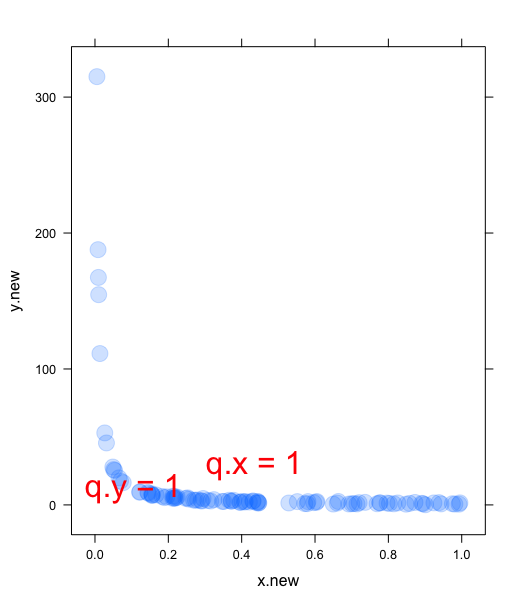
\includegraphics[width=.9\linewidth]{E7_3-9.png}  
  \caption{ }
  \label{sb7-9}
\end{subfigure}
\begin{subfigure}{.23\textwidth}
  \centering
  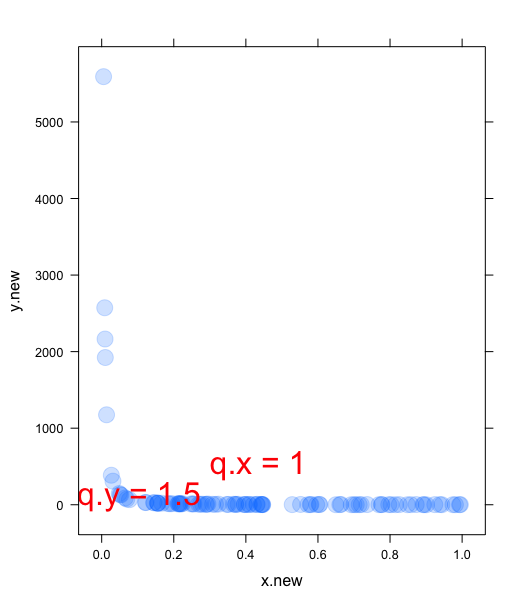
\includegraphics[width=.9\linewidth]{E7_3-10.png}  
  \caption{ }
  \label{sb7-10}
\end{subfigure}
\begin{subfigure}{.23\textwidth}
  \centering
  \includegraphics[width=.9\linewidth]{E7_3-11.png}  
  \caption{ }
  \label{sb7-11}
\end{subfigure}
\begin{subfigure}{.23\textwidth}
  \centering
  \includegraphics[width=.9\linewidth]{E7_3-12.png}  
  \caption{ }
  \label{sb7-12}
\end{subfigure}
\newline
\begin{subfigure}{1\textwidth}
  \centering
  \includegraphics[width=.22\linewidth]{E7_3-13.png}  
  \caption{ }
  \label{sb7-13}
\end{subfigure}
\caption{Iterations of the different values of lambda for the Tukey ladder of powers for the exponential equation.}
\label{fig7}
\end{figure}

Seeing Figure \ref{fig7} we see that the closer linear plot is between the values of Figure \ref{sb7-6} and Figure \ref{sb7-7}, so instead of showing the value of $\lambda$ = 3, we plot the value between $\lambda$ = -0.5 and $\lambda$ = 0, and in Figure \ref{sb7-13} we use the $\lambda$ = 0.25. This shows to be the more linear in counts of behavior. \\

\clearpage

\subsection{Logarithmic}

In this case, because of the logarithmic properties, \texttt{x} must be $>$ to 0. Equation \ref{eq4} shows the parameters used, 

\begin{equation} \label{eq4}
y = a + b * log(x)
\end{equation} 

where b is the parameter that determines the shape of the plot, and there are the same fixed variables used in the polynomial, quadratic and exponential experiments.\\

\begin{figure}[]
\begin{subfigure}{.3\textwidth}
  \centering
  \includegraphics[width=.9\linewidth]{Ej7_p4-1.png}  
  \caption{ }
  \label{sb8-1}
\end{subfigure}
\begin{subfigure}{.3\textwidth}
  \centering
  \includegraphics[width=.9\linewidth]{Ej7_p4-2.png}  
  \caption{ }
  \label{sb8-2}
\end{subfigure}
\begin{subfigure}{.3\textwidth}
  \centering
  \includegraphics[width=.9\linewidth]{Ej7_p4-3.png}  
  \caption{ }
  \label{sb8-3}
\end{subfigure}
\caption{Scatter plot of equation (a), Residuals vs. Fitted plot (b), and Normal Q-Q plot (c) of logarithmic equation.}
\label{fig8}
\end{figure}

\begin{figure}[]
\begin{subfigure}{.23\textwidth}
  \centering
  \includegraphics[width=.9\linewidth]{E7_4-1.png}  
  \caption{ }
  \label{sb9-1}
\end{subfigure}
\begin{subfigure}{.23\textwidth}
  \centering
  \includegraphics[width=.9\linewidth]{E7_4-2.png}  
  \caption{ }
  \label{sb9-2}
\end{subfigure}
\begin{subfigure}{.23\textwidth}
  \centering
  \includegraphics[width=.9\linewidth]{E7_4-3.png}  
  \caption{ }
  \label{sb9-3}
\end{subfigure}
\begin{subfigure}{.23\textwidth}
  \centering
  \includegraphics[width=.9\linewidth]{E7_4-4.png}  
  \caption{ }
  \label{sb9-4}
\end{subfigure}
\newline
\begin{subfigure}{.23\textwidth}
  \centering
  \includegraphics[width=.9\linewidth]{E7_4-5.png}  
  \caption{ }
  \label{sb9-5}
\end{subfigure}
\begin{subfigure}{.23\textwidth}
  \centering
  \includegraphics[width=.9\linewidth]{E7_4-6.png}  
  \caption{ }
  \label{sb9-6}
\end{subfigure}
\begin{subfigure}{.23\textwidth}
  \centering
  \includegraphics[width=.9\linewidth]{E7_4-7.png}  
  \caption{ }
  \label{sb9-7}
\end{subfigure}
\begin{subfigure}{.23\textwidth}
  \centering
  \includegraphics[width=.9\linewidth]{E7_4-8.png}  
  \caption{ }
  \label{sb9-8}
\end{subfigure}
\newline
\begin{subfigure}{.23\textwidth}
  \centering
  \includegraphics[width=.9\linewidth]{E7_4-9.png}  
  \caption{ }
  \label{sb9-9}
\end{subfigure}
\begin{subfigure}{.23\textwidth}
  \centering
  \includegraphics[width=.9\linewidth]{E7_4-10.png}  
  \caption{ }
  \label{sb9-10}
\end{subfigure}
\begin{subfigure}{.23\textwidth}
  \centering
  \includegraphics[width=.9\linewidth]{E7_4-11.png}  
  \caption{ }
  \label{sb9-11}
\end{subfigure}
\begin{subfigure}{.23\textwidth}
  \centering
  \includegraphics[width=.9\linewidth]{E7_4-12.png}  
  \caption{ }
  \label{sb9-12}
\end{subfigure}
\newline
\begin{subfigure}{1\textwidth}
  \centering
  \includegraphics[width=.22\linewidth]{E7_4-13.png}  
  \caption{ }
  \label{sb9-13}
\end{subfigure}
\caption{Iterations of the different values of lambda for the Tukey ladder of powers for the logarithmic equation.}
\label{fig9}
\end{figure}

For the logarithmic equation, in Figure \ref{fig9} we analyze the iterations of lambda and see that Figure \ref{sb9-5} is the one with a linear behaviour, being $\lambda$ = -1.5.\\

\clearpage

\subsection{X with a different distribution.}

For this experimentation we use the Equation \ref{eq5},

\begin{equation} \label{eq5}
y = jitter(x^p, factor = length(x)/2)
\end{equation} 
\begin{description}
\item \texttt{p} is a standard normal random variable,
\item \texttt{x} is a number of 1:100,
\item \texttt{jitter} returns a numeric value of the same lenght as \texttt{x}, but with an amount of noise added in order to break ties.
\end{description}

\begin{figure}[]
\begin{subfigure}{.3\textwidth}
  \centering
  \includegraphics[width=.9\linewidth]{Ej7_p5-1.png}  
  \caption{ }
  \label{sb10-1}
\end{subfigure}
\begin{subfigure}{.3\textwidth}
  \centering
  \includegraphics[width=.9\linewidth]{Ej7_p5-2.png}  
  \caption{ }
  \label{sb10-2}
\end{subfigure}
\begin{subfigure}{.3\textwidth}
  \centering
  \includegraphics[width=.9\linewidth]{Ej7_p5-3.png}  
  \caption{ }
  \label{sb10-3}
\end{subfigure}
\caption{Scatter plot of equation (a), Residuals vs. Fitted plot (b), and Normal Q-Q plot (c) of experiment with different \texttt{x}, and \texttt{y} with a random variable.}
\label{fig10}
\end{figure}

In Figure \ref{fig11} we apreciate that from all the iterations, Figure \ref{sb11-3} is the one showing linear behaviour, with a $\lambda$ = -2.\\

\begin{figure}[]
\begin{subfigure}{.23\textwidth}
  \centering
  \includegraphics[width=.9\linewidth]{E7_5-1.png}  
  \caption{ }
  \label{sb11-1}
\end{subfigure}
\begin{subfigure}{.23\textwidth}
  \centering
  \includegraphics[width=.9\linewidth]{Ej7_5-2.png}  
  \caption{ }
  \label{sb11-2}
\end{subfigure}
\begin{subfigure}{.23\textwidth}
  \centering
  \includegraphics[width=.9\linewidth]{Ej7_5-3.png}  
  \caption{ }
  \label{sb11-3}
\end{subfigure}
\begin{subfigure}{.23\textwidth}
  \centering
  \includegraphics[width=.9\linewidth]{Ej7_5-4.png}  
  \caption{ }
  \label{sb11-4}
\end{subfigure}
\newline
\begin{subfigure}{.23\textwidth}
  \centering
  \includegraphics[width=.9\linewidth]{Ej7_5-5.png}  
  \caption{ }
  \label{sb11-5}
\end{subfigure}
\begin{subfigure}{.23\textwidth}
  \centering
  \includegraphics[width=.9\linewidth]{Ej7_5-6.png}  
  \caption{ }
  \label{sb11-6}
\end{subfigure}
\begin{subfigure}{.23\textwidth}
  \centering
  \includegraphics[width=.9\linewidth]{Ej7_5-7.png}  
  \caption{ }
  \label{sb11-7}
\end{subfigure}
\begin{subfigure}{.23\textwidth}
  \centering
  \includegraphics[width=.9\linewidth]{Ej7_5-8.png}  
  \caption{ }
  \label{sb11-8}
\end{subfigure}
\newline
\begin{subfigure}{.23\textwidth}
  \centering
  \includegraphics[width=.9\linewidth]{Ej7_5-9.png}  
  \caption{ }
  \label{sb11-9}
\end{subfigure}
\begin{subfigure}{.23\textwidth}
  \centering
  \includegraphics[width=.9\linewidth]{Ej7_5-10.png}  
  \caption{ }
  \label{sb11-10}
\end{subfigure}
\begin{subfigure}{.23\textwidth}
  \centering
  \includegraphics[width=.9\linewidth]{Ej7_5-11.png}  
  \caption{ }
  \label{sb11-11}
\end{subfigure}
\begin{subfigure}{.23\textwidth}
  \centering
  \includegraphics[width=.9\linewidth]{Ej7_5-12.png}  
  \caption{ }
  \label{sb11-12}
\end{subfigure}
\newline
\begin{subfigure}{1\textwidth}
  \centering
  \includegraphics[width=.22\linewidth]{Ej7_5-13.png}  
  \caption{ }
  \label{sb11-13}
\end{subfigure}
\caption{Iterations of the different values of lambda for the Tukey ladder of powers for the equation with different \texttt{x} distribution, and \texttt{y} with added noise.}
\label{fig11}
\end{figure}



\clearpage

Figure \ref{fig12} shows the correlations of the different values of lambda working with the different equations used for this work.\\

\begin{figure}[]
\begin{subfigure}{.5\textwidth}
  \centering
  \includegraphics[width=.9\linewidth]{Ej7_boxcox1.png}  
  \caption{$y = a * sqrt(x) + b$ }
  \label{sb12-1}
\end{subfigure}
\begin{subfigure}{.5\textwidth}
  \centering
  \includegraphics[width=.9\linewidth]{Ej7_boxcox2.png}  
  \caption{$y = a*x^2 + b*x + c$}
  \label{sb12-2}
\end{subfigure}
\newline
\begin{subfigure}{.5\textwidth}
  \centering
  \includegraphics[width=.9\linewidth]{Ej7_boxcox3.png}  
  \caption{$y = a * (exp(p * x))  $}
  \label{sb12-3}
\end{subfigure}
\begin{subfigure}{.5\textwidth}
  \centering
  \includegraphics[width=.9\linewidth]{Ej7_boxcox5.png}  
  \caption{$y = jitter(x^p, factor = length(x)/2)  $}
  \label{sb12-4}
\end{subfigure}
\caption{Correlations with the different values of $\lambda$.}
\label{fig12}
\end{figure}


\section{Conclusions}


Starting this work was a bit complicated for me, because I did not fully understand the transformations, but seeing them as an example first helped me understand what it was happening on each iteration. I had to use a built in library to work with the Tukey ladder, and did not use the box-cox transformation, but I think I could grasp the concept of either one a bit better having finished this work.\\


\bibliographystyle{plainnat}
\bibliography{tarea7}


 
\end{document}